% \part{Theoretische Grundlagen und Stand der Forschung}
 
 \chapter{Einstieg}

\largerpage
Die hier vorliegende Untersuchung beschreibt grammatische Strukturen einer fiktionalen Sprache, die auf Imitationen der jiddischen Sprache fußt und zum festen Inventar jüdischer Figurendarstellung im 19. Jahrhundert gehört. Dieses sogenannte \quein{Literaturjiddisch} (\citealt{Richter1995}) ist eine im (langen) 19. Jahrhundert\footnote{Der Terminus \textit{long 19th century} \,%rs? \ili{englisch} oft hochgestellt long 19\textsuperscript{th} century
geht auf den Historiker Eric Hobsbawm (\citeyear{Hobsbawm1962,Hobsbawm1975,Hobsbawm1987}) zurück und bezeichnet den Zeitraum zwischen dem Beginn der Französischen Revolution (1789) und dem Ausbruch des Ersten Weltkriegs (1914).} weit verbreitete literarische Modeerscheinung, ohne die kaum ein literarischer Text auskommt, der mit jüdischen Figuren arbeitet. Dabei fungiert \ili{Literaturjiddisch} vorwiegend im Rahmen des literarischen Antisemitismus (\citealt[vgl.\,][309]{Gubser1998}), wird aber im Verlauf des 19. Jahrhunderts selbst durch jüdische Autoren adaptiert. Dieses Phänomen ist nicht auf die literarische Peripherie zu beschränken, sondern findet sich auch in kanonischen Texten wie z.\,B.\, Büchners \qu{Woyzeck} (1836–1837), Gustav Freytags \qu{Soll und Haben} (1855) oder Thomas Manns \qu{Wälsungenblut} (1906). Auch ist die sprachliche Markierung jüdischer Figuren kein auf das (lange) 19. Jahrhundert und die deutschsprachige Literatur beschränktes Stilmittel. Man findet diese Strategie bereits im Spätmittelalter und sie ist selbst noch in jüngsten Veröffentlichungen wie Thomas Meyers \qu{Wolkenbruchs wunderliche Reise in die Arme einer Schickse} (2012) oder Sam Apples \qu{Schlepping Through the Alps} (2005) zu finden. Um einen ersten Eindruck von solchen literarischen Bearbeitungen der jiddischen Sprache zu geben, ist hier die handschriftlich überlieferte \qu{Judenpredigt} (1856) Goethes als eines der prominenteren Beispiele angeführt: 
 
 \begin{quote}

Judenpredigt.\\
Sagen de Goyen, wer hätten kä König, kä Käser, kä Zepter, kä Kron’; do will ich äch aber beweise, dass geschrieben stäht: dass wo habend äh König, äh Käser, äh Zepter, äh Kron’. Aber wo haben wir denn unsern Käser? Das will ich äch och sage. Do drüben über de grose grause rote Meer. Und do wäre dreimall hunnerttausend Johr vergange sei, do werd’ äh groser Mann, mit Stiefle und Spore grad’ aus, sporenstrechs gegange komme übers grose grause rote Meer, und werd in der Hand habe äh Horn, und was denn vor äh Horn? Aeh Düt-Horn. Und wenn der werd ins Horn düte, do wären alle Jüdlich, die in hunnerttausend Johr gepöckert sind, die wären alle gegange komme ans grose grause rote Meer. No’, was sogt ehr dozu? Un was äh gros Wonner sei werd, das will ich äch och sage: Er werd geritte komme of äh grose schneeweise Schimmel; un was äh Wonner, wenn dreimal hunnert un neununneunzig tausend Jüdlich wäre of den Schimmel sitze, do wären se alle Platz habe, un wenn äh enziger Goye sich werd ach drof setze wolle, do werd äh kenen Platz finne. No, was sogt ehr dozu? Aber was noch ver äh groser Wonner sei werd, das will ich äch och sage: Un wenn de Jüdlich alle wäre of de Schimmer sitze, do werd der Schimmel kertzegerode sein grose, grose Wätel ausstrecke, do wären de Goye denken: kennen wer nich of de Schimmel, setze wer uns of de Wätel. Un denn wäre sich alle of de Wätel nuf hocke. Un wenn se alle draf setzen, und der grose schneeweise Schimmel werd gegange komme dorchs grause rote Meer zorick, do werdd äh des Wätel falle lasse, und de Goye werde alle ronder falle ins grose grause rote Meer. \\ No, was sogt ehr dozu?
%\begin{flushright}
 (\citealt[1086]{GoetheJudenpredigt}; Erstdruck 1856 im Weimarischen Sonntagsblatt Nr. 50, S.\, 418f.) %\end{flushright}
  \end{quote}

\largerpage
\noindent Der Text lebt hauptsächlich von den vorgenommenen Manipulationen der deutschen Schriftsprache. Ohne diese Manipulationen würde sich dieser Text keinem Leser (des 19. Jahrhunderts) als fiktionale Äußerung eines Juden erschließen. Diese Abweichungen vom Schriftdeutschen lassen sich in weit verbreitete dialektale Elemente (z.\,B.\, \textit{n}/\textit{e}-Ausfall \textit{beweise}, \textit{grad’ aus}, oder charakteristisch rheinfränkische Dialektmerkmale wie in \textit{Düt-Horn}) und in jiddische Elemente beschreiben und unterteilen. Letztere zeigen aus dem im deutschsprachigen Raum gesprochenen Westjiddischen bekannte Strukturen,  wie etwa der Diminutiv Plural \textit{Jüdlich}, die Verwendung des \isi{Hebraismus} \textit{Goye} \sem{Nicht-Juden} oder die Diphthongierung von {\mhd} \textit{ô} > {\wj} \textit{au}/\textit{ou} \textit{grause}. Die vorliegende Arbeit stellt auf der Grundlage eines \isi{Korpus} von 63 Texten dar, welcher sprachlichen \,%rs Adjektivendung
Phänomene sich das Literaturjiddische bedient, und setzt diese in Beziehung mit Daten jiddischer und deutscher Dialekte. Die hier analysierten Texte sind überwiegend antisemitischer kultur- und literaturgeschichtlicher \textit{Junk}, der bislang kaum sprachwissenschaftliches oder literaturwissenschaftliches Interesse geweckt hat. Doch selbst diese \textit{zweit-} und \textit{drittklassige} Literatur stellt ein interessantes historisches Zeugnis dar. Der linguistische Wert einer deskriptiven Perspektive auf eine fiktionale Sprache ist vielfältig (vgl.\, Abschnitt \ref{lijisprachwissenschaft}, S.\, \pageref{lijisprachwissenschaft}). Insbesondere können solcherlei Daten einen Beitrag dazu leisten, die noch weitgehend unerforschte grammatische und soziolinguistische Situation des späten Westjiddischen zu erfassen. Darüber hinaus bieten sie als Zeugnis sprachlicher \isi{Imitation} Einblicke in Grundmechanismen von Spracherwerb und \isi{Sprachkontakt}. 


\section{Ziele der Arbeit}\label{ziele}	
  
Die Idee zu dieser Arbeit entwickelte sich aus den ersten sich abzeichnenden Ergebnissen des DFG-Projekts \qu{\ili{Westjiddisch} im (langen) 19. Jahrhundert} an der Philipps-Universität Marburg. An den Grundansatz des Projektes, Quellen zum späten Westjiddischen \,%rs Endung
ausfindig zu machen, ist auch das Kernziel dieser Arbeit geknüpft: Es soll geprüft werden, inwieweit literaturjiddische Texte Aufschluss über die westjiddische Sprachrealität geben können.

Wie ich bereits in meiner Bachelor- und Masterarbeit (\citealt{Schaefer2008} und \citeyear{Schaefer2010}) zeigen konnte, sind literarische %\footnote{In dieser Arbeit wird der Begriff \quein{literarisch} im aristotelischen Sinne zur Bezeichung literarischer Texte der drei Gattungen Prosa, Lyrik, Drama verwendet.} 
Texte nicht zwangsläufig  ungeeignete Sprachzeugnisse. \,%rs z klein + s 
Sie können zwar, wie die meisten historischen Zeugnisse, \,%rs Zeugnisse
nur positive Evidenz liefern. Verbindet man aber Basiswerkzeuge der Literaturanalyse mit linguistischer Empirie, bergen solche Texte sogar große Zugewinne für die soziolinguistische, diskurs- und kulturgeschichtliche Situation einer Sprache. Ein weitestgehend im Hintergrund verfolgtes Ziel dieser Arbeit wird damit auch immer die Validierung literarischer Texte als sprachhistorische Quelle sein.

Literaturjiddische Texte unterscheiden sich in einem entscheidenden Punkt von den üblichen sprachhistorischen Quellen: Sofern es sich um Texte nicht-jüdischer (oder zumindest nicht jiddisch-muttersprachlicher) Autoren handelt, sind diese Texte keine Primärquellen einer Varietät, sondern Sekundärquellen, die auf Laienkonzepten beruhen. Was zunächst als ein großes Manko erscheint, ist bei genauerer Betrachtung ein Bonus des Materials. Damit werden erstmals historische Imitationsdaten erhoben und analysiert. Die dabei zu klärenden Fragen sind, wie genau die Imitationen des Jiddischen funktionieren, ob aufgrund der allen Texten gemeinsamen Rahmensprache (Deutsch) auch formale Gemeinsamkeiten der angewandten Mittel zur \isi{Imitation} bestehen und ob sich der Rückgang des Westjiddischen im Laufe des 19. Jahrhunderts auch in den Laienkonzepten bemerkbar macht.

Ein sich daran anschließender Aspekt dieser Arbeit besteht darin, den Diskurs des Jiddischen im deutschsprachigen Raum anhand von literarischen Quellen abzustecken und näher zu verstehen. Mittels ausgewählter Quellen zeigt diese Arbeit, wie sich die externe Wahrnehmung jüdischer Sprachen und speziell des Jiddischen im Laufe der Geschichte verändert hat bzw. in welchen Bereichen sie stabil geblieben ist. Es können drei Stadien dieses Diskurses identifiziert werden (vgl. Kapitel \ref{lijiliteraturwissenschaft}): 



\begin{enumerate}
\item \ili{Literaturhebräisch} (\hai{{\LiHe}}): Die Auseinandersetzung mit dem Hebräischen in Passionsspielen aus dem 14. bis 16. Jahrhundert. \\
\item \ili{Literaturjiddisch} 1 (\hai{{\LiJi}1}): Die sprachliche Markierung jüdischer Figuren als Stilmittel zur literarischen Darstellung %im Prozess des Ausschlusses des Jiddischen %im sich formierenden Gedanken einer deutschen Schreibvarietät (Standardsprache) 
im (langen) 19. Jahrhundert.\\ % Jiddisch ist in diesem Stadium noch eine vitale Varietät und fester Bestandteil des deutschen Varietätengefüges. \\
\item \ili{Literaturjiddisch} 2 (\hai{{\LiJizwei}}) und \ili{Filmjiddisch} (\hai{{\FiJi}}): Die sprachliche Markierung jüdischer Figuren als Stilmittel zur literarischen Darstellung im späten 20. und frühen 21. Jahrhundert in der deutsch- und englischsprachigen Literatur und im Film.\\ %Zu diesem Zeitpunkt ist Jiddisch nicht mehr Mehrheitssprache der in deutschsprachigen Ländern lebenden Juden. \\
 \end{enumerate}
   
\noindent  Das erste Stadium wird lediglich in einem Überblick über die Forschungslage angeschnitten (Abschnitt \ref{lihe}, S.\, \pageref{lihe}). Erst das zweite Stadium wird unter sprachwissenschaftlichen Gesichtspunkten auf Grundlage eines umfangreichen \isi{Korpus} analysiert (Teil \ref{analysen}, S.\, \pageref{analysen}). Das dafür herangezogene Textkorpus des \hai{{\LiJieins}} ist ein Auszug aus den im Marburger \ili{Westjiddisch}-Projekt aufgefundenen Quellen (vgl.\, Abschnitt \ref{kernkorpus}, S.\, \pageref{kernkorpus}). Die Fassung der zurgundeliegenden Dissertationsschrift beinhaltet ein drittes Teilkorpus mit Texten der Gegenwartsliteratur. Dieses zeigt, wie sich die Muster des Literaturjiddischen in der Sprach- und Mediensituation des 21. Jahrhunderts entwickelt haben. Zu diesem dritten Stadium wurden in \textcite{SchaeferDiss} exemplarisch 7 ($+$ 2 englischsprachige) \,%rs englischsprachig
  Texte des \hai{{\LiJizwei}} analysiert. Die vorliegende Publikation beschränkt sich jedoch auf die Darstellung der Situation im 18. und 19. Jahrhundert und fasst nur die zentralsten Ergebnisse aus der Analyse der Quellen zum \hai{{\LiJizwei}} in Kapitel \ref{phaenomene} zusammen.  Das Verhältnis zum Film wird ebenfalls nur in einem kurzen Exkurs thematisiert (Abschnitt \ref{fiji}, S.\, \pageref{fiji}). Das Hauptaugenmerk liegt damit eindeutig auf dem zweiten Stadium und damit auf dem (langen) 19. Jahrhundert, einer Periode, in der wir noch von einem relativ vitalen Westjiddischen ausgehen können und die daher von besonderem Interesse ist, da sie noch in eine Zeit fällt in der man von einem Deutsch-Jiddischen Sprachkontakt ausgehen kann.
 

\section{Begriffsdefinitionen}\label{begriffsdefinitionen}
 \largerpage
Die unterschiedliche Verwendung verschiedener Begriffe, insbesondere die der Sprachbenennungen, sorgt innerhalb der Jiddistik immer wieder für Missverständnisse. Auch verwendet diese Arbeit einige Termini mit einer wenig etablierten Bedeutung. Aus diesem Grund sollen im Folgenden kurze Definitionen der zentralen Begrifflichkeiten dieser Arbeit angegeben werden. 

\begin{itemize}
\item \quein{Westjiddisch} bezeichnet jiddische Varietäten und historischen Sprachstufen, die mit diversen deutschen Varietäten in direktem \isi{Sprachkontakt} standen und keinem koterritorialen Kontakt zu slawischen Sprachen ausgesetzt waren. 
Der vielfach gebrauchte und unterschiedlichst verwendete Begriff \quein{Jüdisch-Deutsch} (vgl.\, u.\,a.\, \citealt{Simon1988,Weinberg1973,Weinberg1981,Lowenstein1979}; erstmals  \citealt{Wagenseil1699}) wird in dieser Arbeit zur Bezeichnung dieser Varietät nicht verwendet, es sei denn in zitierter Form. Dasselbe gilt für andere Sprachbenennungen des (West"~)Jiddischen (vgl.\, \citealt[3–9]{Weinreich1923}).
\item \quein{Ostjiddisch} bezeichnet hingegen alle jiddischen Varietäten und historischen \mbox{Sprachstufen}, die mit v.\,a.\, slawischen  Varietäten in koterritorialem Kontakt standen. Die Begriffe \quein{Ostjiddisch} und \quein{Westjiddisch} stehen damit ausschließlich in einer sprachgeographischen, nicht aber in einer diachronen Relation zueinander.
\item Die \isi{Periodisierung} der verschiedenen Sprachstufen folgt prinzipiell \cite[719--733]{Weinreich1973}: 


%\begin{chronology}[50]{1200}{1999}{3ex}[\textwidth]
%\event[1200]{1500}{\small{Altjiddisch}}
%\event[1500]{1700}{\small{Mitteljiddisch}}
%\event[1700]{1950}{\small{Spätes Westjiddisch}}
%\event[1700]{1999}{\small{modernes Ostjiddisch}}
%\end{chronology} 
%% zeitleiste: grauer Bereich ist zu klein und wird daher nicht angezeigt u. Lösung für Überlappung von spät. \ili{WJ} und mod. \ili{OJ}?!



\begin{itemize}
\item  \quein{Altjiddisch} ({\aj}) bezeichnet demnach die Periode ab ca.\, 1250 bis ca.\, 1500
\item  \quein{Mitteljiddisch} ({\mj}) von ca.\, 1500 bis ca.\, 1700
\item  \quein{Spätes Westjiddisch} und \quein{modernes Ostjiddisch}/\quein{Standard-Ost"-jiddisch} (\quein{New Yiddish} bei \citealt[719--733]{Weinreich1973}) ab ca.\, 1700
\end{itemize}
Die Zeit von ca.\, 1000 bis ca.\, 1250 kann als  \quein{Vorgeschichte des Jiddischen} bezeichnet werden, aus der uns keine Quellen überliefert sind. 

\largerpage
\item Die germanistische Dialektologie ist ein Kind des 19. Jahrhunderts und entwuchs neben der Grimmschen Idee des Sammelns hauptsächlich der Mode dieser Zeit, kartographische Verfahren auf soziokulturelle Lebensbereiche anzuwenden (vgl.\, \citealt[89–107]{SchmidtHerrgen2011}; \citealt{Schneider2004}). Der Sprachraum ist für die Dialektologie eine notwendige Dimension, sofern Varietäten ausschließlich aufgrund ihrer diatopischen Gemeinsamkeiten (\isi{Isoglossen}) und im Kontrast zu einer Sprachnorm (Standardsprache) definiert werden. In der klassischen Dialektologie  sind Dialekte \qu{die standardfernsten, lokal oder
kleinregional verbreiteten Vollvarietäten} (\citealt[57]{SchmidtHerrgen2011}).
Diese Definition mag für die Situation deutschsprachiger Varietäten des 19. und 20. Jahrhunderts sinnvoll gewählt sein, kann jedoch nicht auf das Jiddische angewandt werden, welches weder in einem Bezugssystem zu einer Schriftnorm vergleichbar der Situation im Deutschen steht, noch zeigt es so kleinräumige Variation wie das Deutsche. Gleiches gilt für deutsche und jiddische Varietäten älterer Sprachstufen. Daher verwendet diese Arbeit die in der deutschsprachigen Dialektologie eher unkonventionelle Dialektdefinition von Helmut Weiß (\citeyear[1--15]{Weiss1998}, \citeyear{Weiss2009}): \qu{A dialect consists of groups of mutually comprehensible \hai{I}-languages.} (\citealt[257]{Weiss2009}). Weiß (\citeyear{Weiss1998}) unterscheidet zusätzlich zwischen zwei Typen von \hai{I}-Sprachen: 
\begin{itemize}
\item [(A)] \hai{N1}-Sprachen (sprich: natürliche Sprachen erster Ordnung) sind unmittelbare Derivate von \hai{I}-Sprachen, die das \hai{L1}-Kriterium des muttersprachlichen Erwerbs erfüllen.
\item [(B)] \hai{N2}-Sprachen (sprich: natürliche Sprachen zweiter Ordnung) sind mittelbare Derivate von \hai{I}-Sprachen, die das \hai{L1}-Kriterium nicht erfüllen.\\ 
(\citealt[3]{Weiss1998})
\end{itemize}

Damit gilt jede Varietät, die muttersprachlich erworben wird ({\oj} \textit{mame-loshn}), demzufolge als Dialekt. Elegant an dieser Definition ist besonders, dass ein Dialekt  nicht zwangsläufig in einer bipolaren Beziehung zu einer überdachenden Standardsprache ({\oj} \textit{klal-shprakh}) stehen muss.\\
Auch wenn dieser Dialektbegriff den Grundkonzepten der klassischen Dialektologie nicht entspricht, werden deren Ergebnisse zur räumlichen Variation deutscher Varietäten 
und die daraus resultierende Einteilung der deutschen %\todo{definit for hyphenation}
 \quein{Basisdialekte} ($=$ synchroner, 
% überwiegend
hauptsächlich
phonologischer Zustand der dt.\, Dialekte des späten 19. und frühen 20. Jhs.) auf Grundlage ihrer diatopischen Eigenschaften aus praktischen Gründen beibehalten. In dieser Arbeit wird die Einteilung der deutschen Basisdialekte nach Peter Wiesinger (\citealt{Wiesinger1983a}) verwendet (vgl.\, Abbildung \ref{kartedtdialekte}). 


% \todo{richtig als farbgrafik eingestellt?}
%%%%Karte Dialekte%%%%
\begin{figure}[h!]
 \farbgrafik
\centering

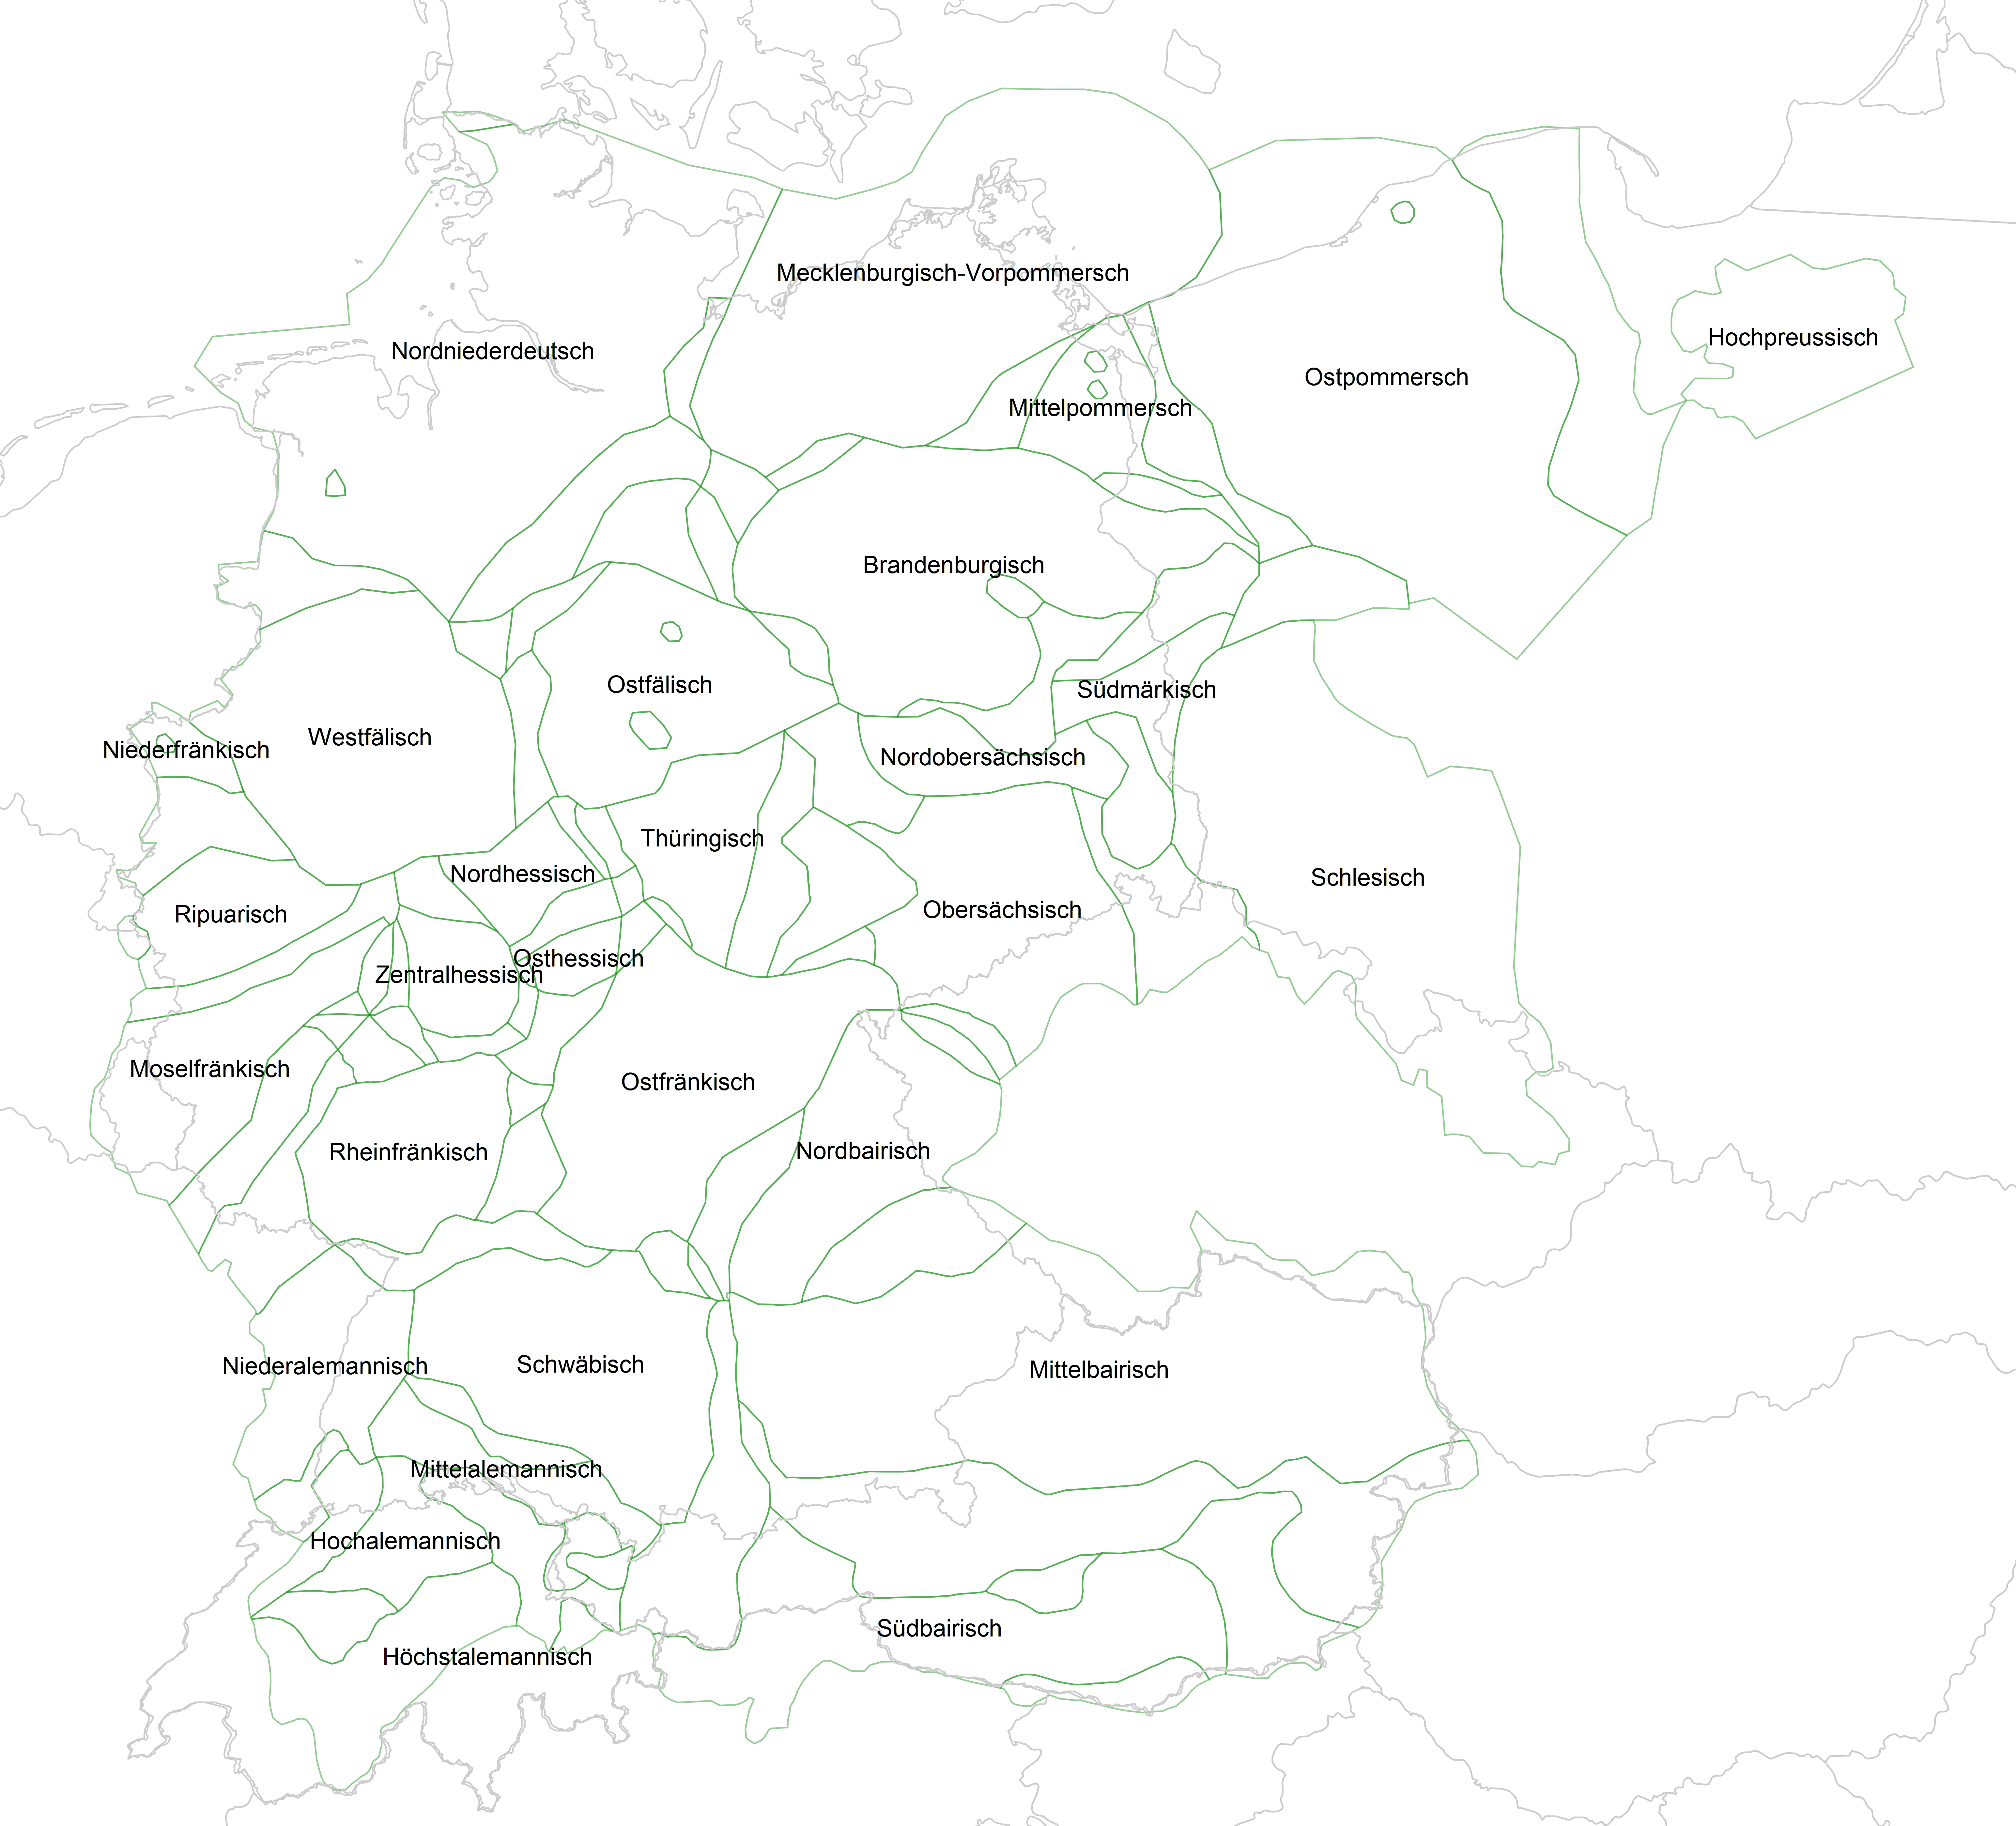
\includegraphics[width=\textwidth]{figures/WiesingerREDE2.png}
		\caption{\label{kartedtdialekte}Einteilung deutscher Dialekte (ohne Sprachinseln) nach \parencite[830, Karte 47.4]{Wiesinger1983a}; erstellt mit \url{www.regionalsprache.de/}}
	\end{figure}



\item Da der verwendete Dialektbegriff nicht in einer direkten Abhängigkeit zu einer \quein{Standardsprache} steht, ergibt sich auch ein in der deutschsprachigen Dialektologie eher unüblicher Standardbegriff. Als \quein{Standardsprache} wird zunächst nach Haugen (1994) jede schriftsprachliche Norm verstanden:

\begin{quote}
Any vernacular (language or dialect) may be \sem{standardized} by being given a uniform and consistent norm of writing that is widely accepted by its speakers. It may then be referred to as a \sem{standard} language. \parencite[4340]{Haugen1994}
\end{quote}

 
Diese Definition, die Aussprachenormen zunächst nicht mit einbezieht, ist besonders für die historische Perspektive sinnvoll, da wir bis in das \,%rs in das
20. Jahrhundert hinein von einer Parallelität von Dialekten und Schreibvarietäten ausgehen können. Die Entstehung einer überregionalen Schreibnorm, die zumeist auch nationalbildend wirkt, ist ein dynamischer Prozess. Das moderne Schriftdeutsche entwickelt \,%rs entwickelt 
sich ab dem 16. Jahrhundert (vgl.\, \citealt{Besch1988,Besch2003,Mattheier2000}). Für das (lange) 19. Jahrhundert als relevanten Zeitraum der vorliegenden Untersuchung kann man bereits von einer weitaus gefestigteren Schreibnorm ausgehen als in früheren Jahrhunderten; nichtsdestotrotz muss jedoch bedacht werden, dass der Standard des 19. Jahrhunderts noch in vielerlei Hinsicht ein im Vergleich zum Gegenwartsdeutschen \,%rs +en
des 21. Jahrhunderts inhomogenes, präskriptives \,%rs präskriptives
System darstellt (vgl.\, \citealt{Elspass2005a,Elspass2005}). Der Normbegriff der Autoren des (langen) 19. Jahrhunderts unterscheidet sich von der heutigen Form und Funktion präskriptiv genormter Register. Nach der Definition von Weiß (s.\,o.) macht die deutsche Standardsprache im Verlauf des 19. und frühen 20. Jahrhundert einen Wandel vom Typ \hai{N2} zum Typ \hai{N1} durch (vgl.\, \citealt[12f]{Weiss1998}). 


\item Die Einteilung jiddischer Dialekte folgt grundsätzlich derjenigen von \citealt{Katz1983}. Da die Katz'sche Einteilung der westjiddischen Dialekte durch kaum empirische Evidenz gestützt ist, nimmt diese Arbeit zur Verfeinerung des Dialektraums eine zusätzliche  Ost-West-Einteilung entlang des 9. Längengrads (Hamburg–Bregenz) vor.\label{BregenzHH} Diese Grenze verläuft entlang der \ili{bairisch}–alemannischen Sprachgrenze sowie der zwischen Ost- und Westmittel- \linebreak deutsch und der zwischen den west- und ostniederdeutschen Dialekten (vgl.\, \citealt{Wiesinger1983a}). 
% Damit orientiert sich diese Einteilung an den Raumstrukturen deutscher Dialekte, selbst wenn empirische Befunde zu einer solchen geographischen Gliederung des Westjiddischen bislang nicht erbracht werden konnten.
Damit orientiert sich diese Einteilung an den Raumstrukturen deutscher Dialekte, selbst wenn empirische Befunde zu einer solchen geographischen Gliederung des Westjiddischen bislang nur für den nördlichen Raum entlang der Elbe erbracht werden konnten (vgl. \citealt[209]{Ramer1997}). 
Daraus ergeben sich die westjiddischen Dialektregionen: 
westliches \ili{Südwestjiddisch} (westl. \hai{{\SWJ}}), 
östliches \ili{Südwestjiddisch} (östl. \hai{{\SWJ}}), 
westliches Zentral\ili{westjiddisch} (westl. \hai{{\ZWJ}}), 
östliches Zentralwest\-jid\-disch (östl. \hai{{\ZWJ}}), 
westliches \ili{Nordwestjiddisch} (westl. \hai{{\NWJ}}) und 
östliches \ili{Nordwestjiddisch} (östl. \hai{{\NWJ}}). 
Die Übergangsgebiete \ili{südliches Übergangsjiddisch} (\hai{{\SÜJ}}) und \ili{nördliches Übergangsjiddisch} (\hai{{\NÜJ}}) sowie die ostjiddischen Dialekte (Zentral\ili{ostjiddisch} ‏\hai{{\ZOJ}}, Süd\ili{ostjiddisch} \hai{{\SOJ}} u. \ili{Nordostjiddisch} \hai{{\NOJ}})  folgen weiterhin Katz (\citeyear{Katz1983}). 

%%%%Karte Dialekte%%%%
\begin{figure} 
\centering
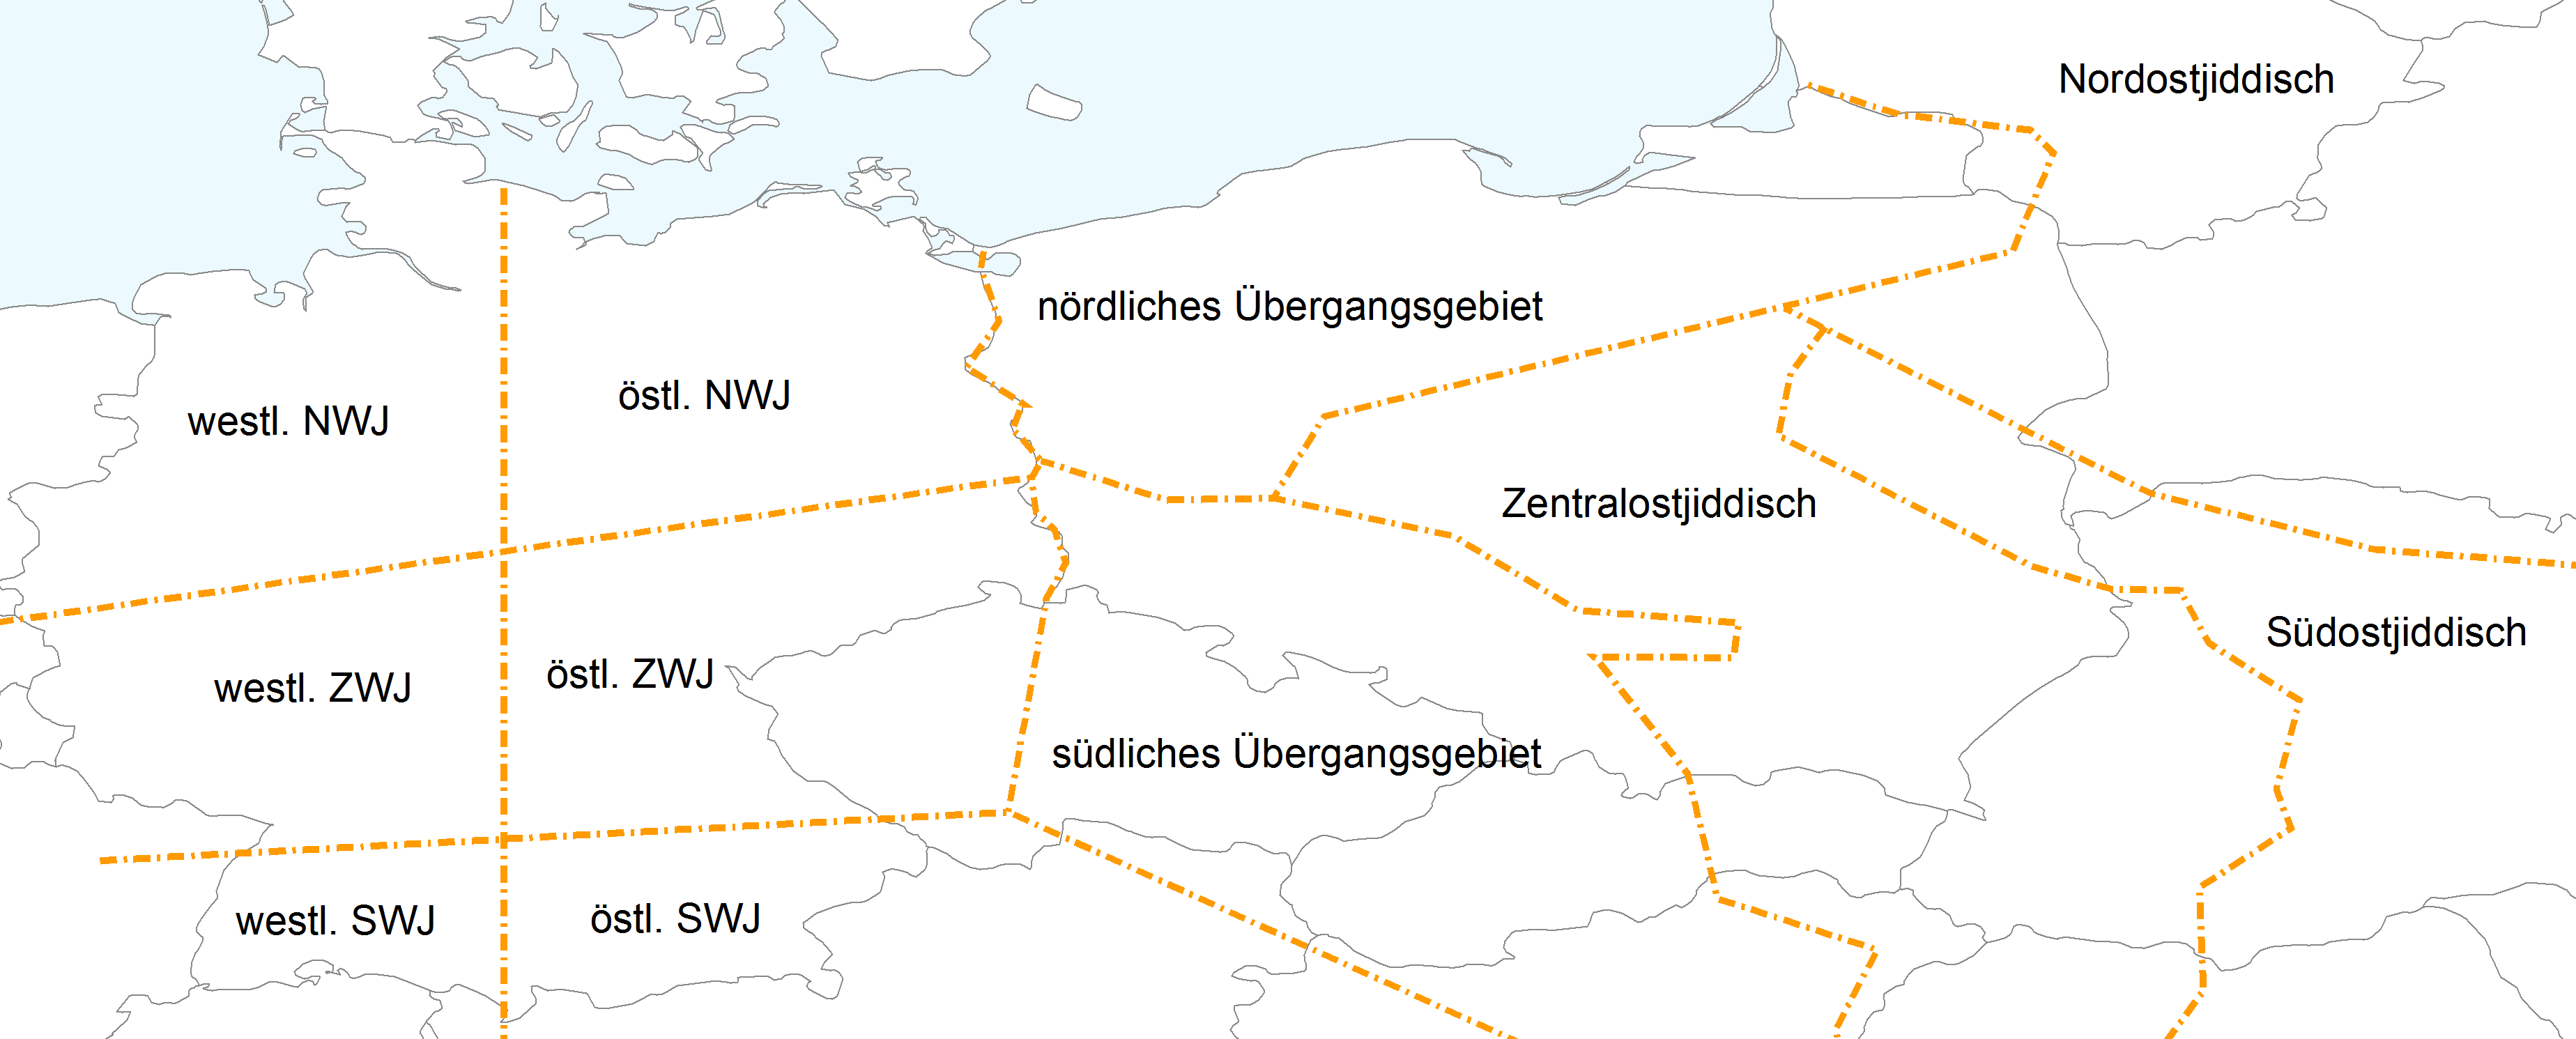
\includegraphics[width=\textwidth]{figures/regionen_diss_farbe2b.png}
		\caption{\label{karteregionen}Einteilung jiddischer Dialekte in Anlehnung an \cite{Katz1983}}
		\end{figure}
 
		%\clearpage

\newpage 	
\item Ein für diese Arbeit zentraler Begriff ist derjenige der \quein{Imitation}. Sprachliche \isi{Imitation} wird als genereller Oberbegriff für die Nachahmung einer Sprache durch einen Nicht-Muttersprachler verwendet. Die genauen Strategien, wie diese \isi{Imitation} vollzogen wird, beschreiben die Begriffe \quein{Emulation} und \quein{Simulation}. Im Falle der \isi{Emulation} wird die zu imitierende Sprache (target language, Zielsprache) in ein bestehendes Grundsystem (Grammatik) einer Matrixsprache eingebettet, adaptiert.\footnote{Der Begriff \quein{Matrixsprache} ist in Anlehnung an das \textit{matrix language frame model} (\hai{MLF}) nach 
\citeauthor{MyersScotton1993} (\citeyear{MyersScotton1993,MyersScotton2002}) gewählt, welches ein ideales Modell für die Grundstrukturen bilingualer Interferenzen wie code-switching 
oder code-mixing darstellt, indem es von einer asymmetrischen Opposition von \textit{matrix language} und \textit{embedded language} ausgeht. Sprachliche \isi{Imitation} ist insofern mit Bilingualismus vergleichbar, als dass ein Ausgleich zwischen zwei Sprachen stattfindet, in welchem eine Sprache (\textit{matrix language}) die Basis bildet, die entweder gezielt (emulierende \isi{Imitation}) oder spontan (code-switching) 
durch eine weitere Sprache (\textit{target language} oder \textit{embedded language}) manipuliert wird. Der größte Unterschied besteht darin, dass die in die Matrixsprache eingebundene Sprache im Fall von Bilingualismus vollständig beherrscht wird, im Fall der \isi{Imitation} jedoch bestenfalls einzelne Strukturen bekannt sind. Aus diesem Grund wird zwar Myers-Scottons (\citeyear{MyersScotton1993,MyersScotton2002}) Begriff der Matrixsprache adaptiert, auf eine Verwendung (und Eindeutschung) des Begriffs \textit{embedded language} wird aber  verzichtet. Es wird hier vielmehr die Terminologie Myers-Scottons verwendet, als ihr Modell. Es ist weiteren Arbeiten vorbehalten zu prüfen, \,%rs  prüfen,
ob die Mechanismen von sprachlicher \isi{Imitation} denen von code-switching/code-mixing folgen.\,%rs hier klein s.o.
} Die \isi{Simulation} einer Sprache hingegen erfolgt losgelöst von einem Grundsystem.
Die Graphiken in Abbildungen \ref{emulativgrafik}  und \ref{simulativgrafik} illustrieren den grundlegenden Unterschied zwischen simulierender und emulierender \isi{Imitation}. Im Fall sprachlicher \isi{Emulation} werden erkannte Strukturen der Zielsprache in das System der Matrixsprache integriert. Die sprachliche \isi{Simulation} hingegen integriert lediglich oberflächliche Strukturen der Zielsprache in das System der Matrixsprache und so treten Formen der Zielsprache losgelöst von einer sprachlichen Struktur auf. In anderen Worten: die \isi{Simulation} verfügt im Gegensatz zur \isi{Emulation} über keine zugrundeliegenden sprachlichen Strukturen, sondern besteht nur aus einzelnen, unzusammenhängenden Formen der Zielsprache. Die qualitative und quantitative Intensität der erkannten Formen wird in beiden Fällen durch einen Filter externer und interner Faktoren bestimmt, der zwischen Matrix- und Zielsprache besteht. Dieser Filter bestimmt die Qualität und Quantität der imitierten Strukturen und entscheidet letzten Endes darüber, welche der Imitationsstrategien (simulativ/emulativ) möglich ist. Er setzt sich aus den folgenden Faktoren zusammen: 
\begin{itemize}
\item [1.] Externe Einflüsse (z.\,B.\, Konzepte von Sprache, Pejorationen, erkannte grammatische Regeln, Intensität des Sprachkontakts) 
\item [2.] Typologische Nähe/Distanz von Matrix- und Zielsprache
\item [3.] Viskosität der Matrixsprache (\,= Potenzial sprachlicher Variabilität und Stativität) 
\end{itemize}
\label{emulationsbegriff}
 Zur weiteren Veranschaulichung helfen Beispiele aus der Architektur. Die sprachliche \isi{Simulation} ist als \quein{Potjomkinsche Dörfer} zu denken; sie ist eine sprachliche Attrappe. Die \isi{Emulation} hingegen kann man mit den Neo-Stilen (Neobarock, Neoromantik, Neorenaissance usw.) des 19. Jahrhunderts vergleichen: An eine moderne Bausubstanz werden Baustile einer anderer Epochen  angebracht, um Historizität zu evozieren. Die Zusammenhänge zwischen Matrix- und Zielsprache und den einzelnen Funktionen und Wirkungsweisen des \quein{Filters} werden im Unterabschnitt \ref{salienz} (ab S.\, \pageref{salienz}) näher ausgeführt. 


\begin{figure}[p]
 \begin{center}
 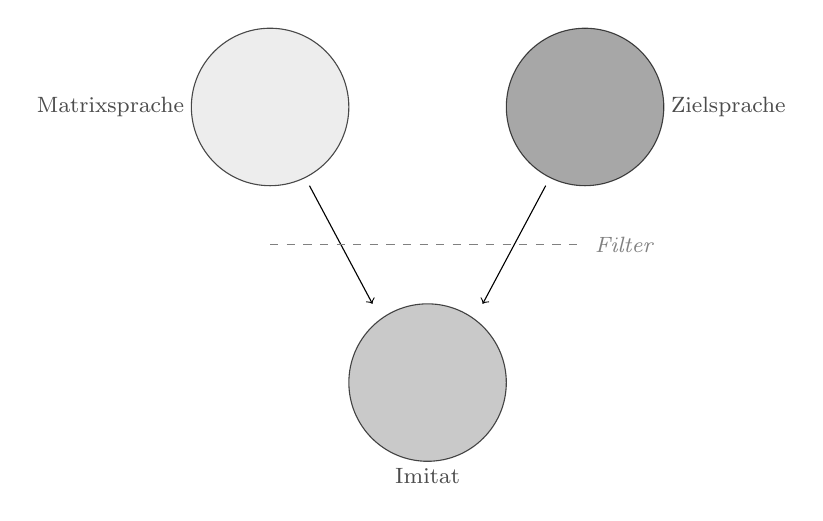
\begin{tikzpicture}
    \draw [fill=gray!20,opacity=0.7](0,1.5) circle (1) node[left=6.4ex] {\footnotesize Matrixsprache};
    \draw [->] (0.5,0.5) -- (1.3,-1);
    \draw [fill=gray!99,opacity=0.7](4,1.5) circle (1) node[right=6.4ex] {\footnotesize  Zielsprache};
        \draw [->] (3.5,0.5) -- (2.7,-1);
        \draw [gray, dashed] (0,-0.25) -- (4,-0.25) node[right] {\footnotesize  \textit{Filter}};
    \draw [fill=gray!60,opacity=0.7] (2,-2) circle (1) node[below=6.4ex] {\footnotesize  Imitat};

             \end{tikzpicture}
              \caption{\label{emulativgrafik}Modell emulativer Imitation}		
\end{center}
 \end{figure}



\begin{figure}[p]
 \begin{center}
 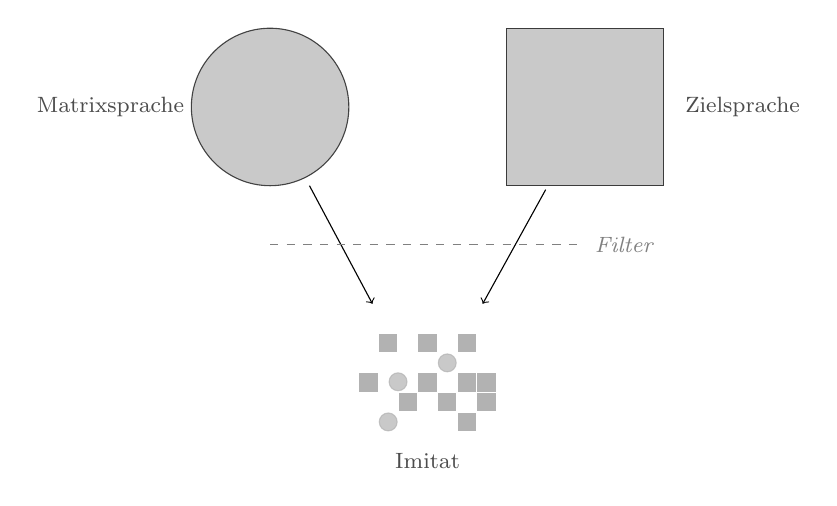
\begin{tikzpicture}
 \draw [fill=gray!60,opacity=0.7](0,1.5) circle (1) node[left=6.4ex] {\footnotesize Matrixsprache};
    \draw [->] (0.5,0.5) -- (1.3,-1);
    \draw [fill=gray!60,opacity=0.7](3, 0.5) rectangle (5,2.5);
 \node[opacity=0.7] at (6,1.5) {\footnotesize  Zielsprache};
          \draw [->] (3.5,0.45) -- (2.7,-1);
             \draw [gray, dashed] (0,-0.25) -- (4,-0.25) node[right] {\footnotesize  \textit{Filter}};
  %  \draw [fill=white!10,opacity=0.7] (2,-2) circle (1) node[below=6.4ex] {\footnotesize  Imitat};
\node[fill=gray!60] at (1.5,-1.5) {};
\node[fill=gray!60] at (2,-2) {};
\node[fill=gray!60] at (2.25,-2.25) {};
\node[fill=gray!60] at (2.5,-2.5) {};
\node[fill=gray!60] at (2.5,-1.5) {};
\node[fill=gray!60] at (2.5,-2) {};
\node[fill=gray!60] at (2,-1.5) {};
\node[fill=gray!60] at (2.75,-2.25) {};
\node[fill=gray!60] at (1.25,-2) {};
\node[fill=gray!60] at (2.75,-2) {};
\node[fill=gray!60] at (1.75,-2.25) {};

\filldraw[color=gray!60,opacity=0.7] (2.25,-1.75) circle (0.75ex);
\filldraw[color=gray!60,opacity=0.7] (1.625,-1.99) circle (0.75ex);
\filldraw[color=gray!60,opacity=0.7] (1.5,-2.5) circle (0.75ex);

\node[opacity=0.7] at (2,-3) {\footnotesize  Imitat};
             \end{tikzpicture}
              \caption{\label{simulativgrafik}Modell simulativer Imitation}	
\end{center}
 \end{figure}


\end{itemize}


\chapter{Forschungsstand}\label{forschungsstand}

In diesem Kapitel wird ein knapper Überblick des derzeitigen Wissensstands der zentralsten Entwicklungen des (West-)Jiddischen und Arbeiten zum Literaturjiddischen gegeben. Da die empirische Datenanalyse im Zentrum dieser Arbeit steht, wurde auf umfangreichere wissenschaftsgeschichtliche Ausführungen zur Jiddistik verzichtet.\footnote{Für den aktuellsten und übersichtlichsten Wissensstand zur Jiddistik seien \cite{AptrootGruschka2010} und für eine detailliertere Darstellung  \cite{Weinreich1973} zurate zu ziehen.}


\section{Übersicht zum Forschungsstand der (west-)jiddischen Sprachgeschichte}\label{westjiddistik}
 
Das wesentliche Charakteristikum des Jiddischen liegt in seiner relativ geringen territorialen Gebundenheit: Jiddisch \qu{was once a vast linguistic continuum, the largest European speech area next to Russian} (\citealt[7]{Weinreich1962}). Während die meisten Sprachen Europas durch politische und geographische Grenzen definiert sind, ist das Jiddische über den religionskulturellen Bund der aschkenasischen Bevölkerung bestimmt, der Diasporajuden Zentraleuropas. Nur wenige andere Sprachen sind so eng an ein ethnisches Konzept gebunden wie das Jiddische an das Judentum.  Wie alle jüdischen Diasporasprachen ist Jiddisch eine Sprache, die immer im Spannungsfeld mit koterritorialen Sprachen stand (vgl.\, \citealt{Spolsky2014}). Jiddische Dialektologie heißt damit auch immer \qu{bilingual dialectology} (\citealt{Weinreich1962}; vgl.\, auch die Arbeiten \citealt{Mieses1915} u. \citealt{Fischer1936}; s.\,a. Kapitel \ref{multilingualismus}, S.\, \pageref{multilingualismus}).

Die jüdisch-aschkenasische Kultur entwickelte sich ab etwa 1000 n.\,d.\,Z. im deutschen Sprachraum, wo \qu{infolge einer sprachlichen Verschmelzung} der mitgebrachten (semitischen und romanischen) Sprachen und mittelhochdeutschen Dialekten das Jiddische entstand (\citealt[1018]{Katz1983}). Jiddische Varietäten, die im Kontakt zu slawischen Sprachen standen (\ili{Ostjiddisch}), entlehnten aus diesen Sprachen zusätzliche Strukturen und Lexeme. In beiden Dialektgroßräumen (Ost- u. \ili{Westjiddisch}) wird aber die überwiegende Komponente des Jiddischen von einer Fusion mittelhochdeutscher Dialekte bestimmt. Dabei handelt es sich aber nicht um eine deutsche Varietät, sondern man muss dem Jiddischen von Beginn an sprachliche Autonomie gegenüber den Geber- und Kontaktsprachen zugestehen. \ili{Westjiddisch} ist im Gefüge der deutschen Varietäten ein eigenständiges sprachliches System: 

\begin{quote}Keine einzige jiddische Mundart deckt sich mit einer bestimmten deutschen Ma. [Mundart; L.S.], sondern das Jiddische ist ein Abklärungsereignis für sich. (\citealt[69; s.\,a. 53–56]{Weinreich1923}) 
\end{quote}

Unser sprachgeschichtliches Wissen über das Alt- und Mitteljiddische ist insbesondere der Forschungsleistung Erika Timms (Universität Trier) zu verdanken. Doch noch immer stehen systematische grammatische Beschreibungen des Alt- und Mitteljiddischen aus, die uns dabei helfen könnten, die älteren Sprachstufen des Jiddischen innerhalb der westgermanischen Sprachen des Spätmittelalters und der frühen Neuzeit zu verorten.\footnote{Hinzu kommt, dass auch unser Wissen über die Nachbarvarietät des Altjiddischen, das tatsächlich gesprochene Mittelhochdeutsch zum jetzigen Zeitpunkt noch äußerst gering ist (vgl.\, \citealt{Wegera2000}).} In der Schriftsprache kann ab frühneuhochdeutscher Zeit eine stärkere Auseinanderentwicklung zwischen Deutsch und Jiddisch beobachtet werden (\citealt{Timm1987b,Timm1991,Timm2005}). Es darf angezweifelt werden, dass diese auch die Mündlichkeit betraf, da sie lediglich Entwicklungen überregionaler Schreibvarietäten erfasst, nicht aber natürlicher Sprachen. Erst mit der nationalistischen und puristischen Sprachpolitik des 19. Jahrhunderts und besonders mit der \isi{Assimilation} des deutschen Judentums löst sich die jahrhundertealte Koexistenz zwischen jiddischen und deutschen Varietäten auf, was vielerorts den \isi{Sprachtod} des Westjiddischen bedeutet. Vereinzelt konserviert blieb die alte Sprachsituation bis ins 20. Jahrhundert hinein in den diglossisch ausgerichteten Gebieten des \hai{{\SWJ}} im Elsass, der Schweiz und daran angrenzenden Ortschaften Südbadens (vgl.\, \citealt[69]{Mieses1915}). Diesem Umstand verdanken wir den umfangreichsten Datenbestand westjiddischer Dialekte (s. Kapitel \ref{chap:quellenkapitel}, S.\, \pageref{chap:quellenkapitel}). 

Der \isi{Sprachtod} des Westjiddischen wird häufig – und analog zum angenommenen Einfluss der lutherschen Bibelübersetzung auf die Standardisierung des Deutschen (vgl.\, \citealt{Besch1999}) – auf Mendelssohns Übersetzung des Tanachs ins Schriftdeutsche mit hebräischen Lettern (1780–1783) und dessen Einstellung zum Jiddischen als einen \qu{Jargon} zurückgeführt (erstmals \citealt[159]{PiererLoebe1860}; \citealt[113–114]{Mieses1915}). Tatsächlich aber sind die Abläufe des jiddischen Sprachtods im deutschsprachigen Raum weitaus komplexer (\citealt[20–32]{Weinreich1923}) und bedürfen einer eingehenden sozialgeschichtlichen Untersuchung. Die Quellenlage zum späten Westjiddischen (vgl.\, Kapitel \ref{chap:quellenkapitel}, S.\, \pageref{chap:quellenkapitel}) spricht dafür, dass sich der Rückgang stufenweise und von Region zu Region abweichend im Laufe des 18., 19. und 20. Jahrhunderts vollzog (vgl.\, \citealt{GuggenheimGruenberg1973,Roemer2002}). 


\section{Linguistische Perspektiven auf Sprachimitation}\label{forschungsgeschichteimitation}
 
Die wissenschaftliche Beschreibung und Untersuchung sprachlicher Imitationen fand bisher in verschiedenen Teilbereichen der Linguistik statt. Besonders in der Spracherwerbsforschung nimmt der behavioristische Ansatz an, dass Erst- und Zweitspracherwerb durch \isi{Imitation} erfolgen (insbes. \citealt{Fraseretal1963,Uzgiris1981}; \citealt[291–294]{Tauten1997}; \citealt{Markham1997,LightbownSpada2006,MeltzoffMoore1977,MeltzoffMoore1983,MeltzoffMoore1989,MetzoffPrinz2002}). Eng verwandt hiermit sind Arbeiten aus dem Feld der Sprachevolution.
 Hier wird das Prinzip des \textit{vocal learning} (\sem{stimmliches Lernen}) als evolutionäre Grundvoraussetzung für sprachliche Kommunikation gesehen (vgl.\, u.\,a.\, \citealt{Fitch2010,HauserChomskyFitch2002,Petkov2012}).\footnote{Vom Menschen abgesehen, findet sich dieses bei Vögeln (u.\,a.\, \citealt{Lipkind2013}), Elefanten (\citealt{Poole2005}), Meeressäugern wie Walen und Robben (\citealt{JanikSlater1997,Ralls1985}) und im Ultraschallbereich bei Fledermäusen (\citealt{Boughman1998}) und Mäusen (\citealt{Arriaga2012}). Bei Primaten konnte bislang ein solches Verhalten nur unter starken Vorbehalten festgestellt werden (\citealt{Crockford2004,Petkov2012}).} Auf einer noch allgemeinneren Ebene sieht das (sozial-)kognitivistische Modell der \qu{Shared intentionality} (erstmals \citealt{Tomaselloetal1993}) von Michael Tomasello und Kollegen in den menschlichen Strukturen und Funktionen von \isi{Imitation} wesentliche Grundprinzipien für  menschliche Lernprozesse – insbesondere die des sozialen Lernens (u.\,a.\,  \citealt[123]{TomaselloCarpenter2007,Tomaselloetal2005,Carpenter2006,Uzgiris1981}). %Problematisch ist hier besonders die Trennung der Bereiche \textit{Sprache} vs. \textit{Musik} (vgl.\, \citealt{Fitch2006}), die z.\,T. graduell zwischen 
 

Durch die gegebene instrumentelle Messbarkeit der lautlichen Ebene ergibt sich, dass phonetische (z.\,T. auch phonologische) \isi{Imitation} bisher stärker untersucht wurde als etwa grammatische (etwa \citealt{Tilmanns2013,Reiterer2012,Nielsen2011,Babel2012}). Das Zusammenspiel aller sprachlicher Ebenen blieb bislang unberücksichtigt. So finden sich auch in den bereits vorhandenen Untersuchungen zu Dialekt- und Akzentimitation nahezu ausschließlich Daten dieser zugänglichen Ebene (etwa \citealt{Babel2011,Purschke2010,Neuhauser2012,Segerup1999,Dossey2012,Siegel2010}; \citealt[12–14, 40]{Trudgill2006}; \citealt{Adank2010}; \citealt[63, 75]{labov1972a}). Eine Ausnahme stellt ein Experiment von \textcite[310–334]{Labov1968_1} dar, wo die \isi{Imitation} eines syntaktischen Phänomens getestet wurde. In ihren \qu{Memory tests} bei  achtjährigen Jungen der sogenannten \textit{Thunderbirds}-Straßengang in New York 1967, untersuchten Labov und seine Kollegen die Spiegelung bzw. \isi{Imitation} der Versuchspersonen von Fällen, \,%rs komma
 in denen  satzfinale Kopulaverben ausfallen.  

In allen 
% bisherigen 
vorliegenden %\todo{bisherigen $\to$ vorliegenden}
Arbeiten wird Dialektimitation vorwiegend als Teilbereich soziolinguistischer (insbesondere Pejoration) oder wahr\-nehmungs\-psycho\-logischer (Salienz) Fragestellungen herangezogen. Wie in Kapitel \ref{lijisprachwissenschaft} (S.\, \pageref{lijisprachwissenschaft}) zu sehen ist, lassen sich Imitationsdaten variationslinguistisch in weiterer Hinsicht vielfach nutzen.


In dieser Arbeit wird erstmals der Versuch unternommen, Sprachimitationen systematisch in \,%rs in 
 den sprachlichen Ebenen Lexik, Phonologie, \isi{Morphologie} und \isi{Syntax}  zu untersuchen. Neu ist dabei der Ansatz, Imitationsdaten auf ihren Nutzen als sprachhistorische Quelle zu prüfen. 
 Von Belang sind hier weniger die psychologischen und neurologischen Grundabläufe, die bei sprachlicher \isi{Imitation} eine Rolle spielen, als vielmehr eine deskriptive Erfassung der grammatischen Elemente, die bei der \isi{Imitation} nah verwandter Varietäten manipuliert werden können. Und so ist auch  die sprachtypologische Perspektive auf Imitationen nah verwandter Varietäten ein Novum. Diese Arbeit betritt somit in vielerlei Hinsicht sprachwissenschaftliches Neuland.
 


\section{Mündlichkeit in der Schriftlichkeit}\label{schmuendlichkeit}

Eine besondere Herausforderung stellt der Datentyp selbst dar. Die dieser Arbeit zu Grunde liegenden Imitationsdaten des (West-)Jiddischen, stammen aus literarischen, zumeist dramatischen, Quellen. Poetische Texte stellen nicht den idealsten Datenquelltyp für linguistische Analysen dar. Zu stark ist ein möglicher Einfluss der poetischen Lizenzen. Vor allem historische Sprachstufen, wie z.B. das Westjiddische des 18. und 19. Jahrhunderts, sind aber zumeist in keiner anderen, \textit{besseren} Form überliefert als der literarischen. Hier gilt die Maxime von  \cite[11]{Labov2010}: \qu{making the best use of bad data}. Dies heißt in der Praxis, die durch poetische Lizenzen entstandenen Strukturen zu identifizieren und aus dem Datenset authentischer Strukturen zu eliminieren. Bei der vorliegenden Untersuchung ist die Situation allerdings anders. Hier stehen die poetischen Lizenzen selbst im Zentrum der Analysen.

Die Verschriftlichung von standardfernen Varietäten ist nicht im Konzept der neuhochdeutschen Schriftlichkeit angelegt. Wenn standardferne Varietäten innerhalb der Literatur auftreten, dann stehen sie immer im Gegensatz zu einer Standardsprache und wirken durch den Kontrast von Schriftlichkeit und Mündlichkeit. 

Es ist
wichtig, %\todo{add wichtig}
 hier zwischen dem \qu{Medium der Realisierung sprachlicher Äußerungen} und der \qu{Konzeption, die die Äußerungen prägt} zu unterscheiden (\citealt[587]{kochoesterreicher1994}). Wenn zum Beispiel ein Dialekt im Rahmen literarischer Figurenrede \,%rs kein Komma
als eine orale Varietät \,%rs kein Komma
verschriftlicht wird, dann ist er vom Medium her schriftlich. Er bleibt dabei aber von der Konzeption her mündlich, ist also nach \cite{KochOesterreicher1985} konzeptionell mündlich. Den Rahmen für konzeptionelle Mündlichkeit innerhalb der medialen Schriftlichkeit literarischer Texte bildet zumeist die direkte Rede. Als Quelle historischer Mündlichkeit eignen sich damit besonders Prosadramen,  wie es z.\,B.\, \textcite{Vosberg2016} am Beispiel einer Analyse von morphosyntaktischen Sprachwandelphänomenen des Englischen bestätigt.

Die hier zu analysierenden Auszüge aus der Figurenrede jüdischer Charaktere sind keine dokumentarischen Aufzeichnungen des gesprochenen Jiddischen, sondern auf Laienwissen fußende Emulationen der Sprache der Autoren (Deutsch) mit eigenen literarischer Funktionen (vgl.\, Kapitel \ref{Kapitel Funktionstypen}). 

Wie genau sprachliche Variation in der Literatur wirkt, dafür liefert Mikhail Bakhkin ein literaturwissenschaftliches Modell. Die unterschiedlichen Sprechlagen und grammatische Möglichkeiten einer Sprache nennt Bakhkin \textit{Heteroglossia}. Diese fließt in einen literarischen Texte ein und  bewirkt einen Diskurs der unterschiedlichen Sprechweisen (\textit{double-voicing}):

\begin{quote}
Heteroglossia, once incorporated into the novel (whatever the forms for its incorporation), is \textit{another's speech in another's language}, serving to express authorial intentions but in a refracted way. Such speech constitutes a special type of  \textit{double-voicing discourse}. It serves two speakers at the same time and expresses simultaneously two different intentions: the direct intention of the character who is speaking, and the refracted intention of the author. In such discourse there are two voices, two meanings and two expressions. \cite[324]{Bakhtin1981}
\end{quote}

\noindent \cite[u.\,a.\, 279, 285, 369, 418]{Bakhtin1981} betont wiederholt, dass ein literarisches Werk erst durch seine internen Dialoge wirkt.\footnote{In der Übersetzung ist hier die Rede von der 
% \textit{Power} 
\qu{Power}
eines Werkes} %\todo{Power nicht kursiv, sondern in ``''} 
Es sind die Abweichungen von der Norm, die poetischen Lizenzen, die einem literarischen Text sprachliche Dynamik verleihen. Die jüdische Figurenrede in der deutschen Literatur ist dafür ein äußerst prägnantes Beispiel. Die große Popularität dieses Stilmittels fußt auf der einfachen und direkten Wirkung, die sprachliche Variation im Rahmen einer sonst normierten Sprache hat. Losgelöst vom Inhalt des Gesagten tritt die Form ins Zentrum und wird somit zum Thema selbst.

 Solche Prinzipien machen sich Texte zu nutzen, die Formen des Literaturjiddischen verwenden. Vor allem im 18. und 19. Jahrhundert haben wir es hier mit Texten zu tun, die nicht in den literarischen Kanon aufgenommen sind und die wenig Komplexität und inhaltliches Gewicht aufweisen. Die Verwendung einer nicht normgerechten Sprache bei jüdischen Charakteren ist zumeist das einzige komische Element dieser Texte. Die Darstellung konzeptioneller Mündlichkeit fungiert hier ähnlich \,%rs kein Komma
 wie das stilisierte \textit{Türkendeutsch} in der Medien- und Jugendkultur der 1990er und frühen 2000er Jahre als \qu{eine Art \textit{fun-code}} (vgl.\, \citealt[59]{Deppermann2007}; \citealt{Auer2003}). Doch \ili{Literaturjiddisch} geht über die humoristische Funktion hinaus. Verwendet von nicht-jüdischen Autoren kann es z.\,B.\, auch identitätsschaffend, nostalgisch wirken (mehr dazu in Kapitel \ref{Kapitel Funktionstypen}).


\chapter{Literarische Traditionen}\label{lijiliteraturwissenschaft}


%\epigraph{\textit{A Huhn, wos kräjt, un a Goi, wos schmusst jiddisch – sollen sein Kapore far mir.}}{--- \textup{Jiddisches Sprichwort (\citealt[524]{Landmann2013})}} 
\largerpage

\noindent Aus der Literaturwissenschaft, insbesondere aus dem Forschungsfeld des literarischen Antisemitismus, liegt uns eine Reihe an Arbeiten zur jüdischen Figurensprache in der deutschsprachigen Literatur vor (insbes. \citealt{FischerBayerd2008,Kremer2007,Schreuder2002,Krobb2000,Glasenapp1999,Gubser1998,Groezinger1998,Richter1995,Och1995,Frey1994,Frey1992,Althaus1981,Althaus1986,Gelber1986,Denkler1977,Jenzsch1974}; erste Ansätze finden sich bereits bei \citealt{Carrington1897}). Dieser Abschnitt zeigt die zentralen Tendenzen auf, die sich aus dem literaturwissenschaftlichen Diskurs für das Literaturjiddische in seinem Verhältnis zum Jiddischen ergeben. Dabei wird der Blick vom Jiddischen in der deutschsprachigen Literatur auf den Umgang mit jüdischen Sprachen generell ausgeweitet. Sinn und Zweck dieses Abschnittes ist es, in einem Überblick die verschiedenen Reflexe, die jüdische Sprachen in literarischen aber auch filmischen Kunstwerken hinterlassen haben, darzustellen.  


\section{Die Sprache jüdischer Figuren als Topos der europäischen Literaturen}\label{euroliji}
%jüdische sprache in anderen literaturen
 
Jüdische Diasporasprachen stehen immer in einer Kontrastbeziehung zu koterritorialen Sprachen. Im Literaturjiddischen wird diese Beziehung literarisch realisiert. So ist es nicht überraschend, dass die besondere jüdische Sprachsituation auch in anderen Literaturen als der deutschsprachigen thematisiert wird. Hebt man die Beschränkung auf die jiddische Sprache auf, so lässt sich in der europäischen Literatur etwas finden, was man als \quein{Literaturjüdisch} bezeichnen kann, da oftmals jüdische Figuren sprachlich markiert werden, jedoch nicht über die jiddische oder hebräische Sprache, sondern über ein generelles \quein{Anders-Sprechen}. Solche Markierungen finden sich zum Beispiel in der
\il{niederdeutsch}niederdeutschen,
\il{dänisch}dänischen,
\il{englisch}englischen, 
\il{polnisch}polnischen  und 
\il{französisch}französischen  Literatur. %format! indizes verursachen leerschlag!!!

In der englischen Literatur kann in den Stücken Marlowes und Shakespeares eine unterschiedliche Sprechweise jüdischer Figuren festgestellt werden (\citealt[193]{Groezinger1998}). Ebenso in Werken des 19. Jahrhunderts, z.\,B.\, von Charles Dickens oder George Eliot (vgl.\, \citealt[193]{Groezinger1998}). Die Thematisierung des Jiddischen selbst tritt m.\,W. jedoch erst ab dem 20. Jahrhundert in der anglo-amerikanischen Literatur in Erscheinung (vgl.\, \citealt{Fischer2003}). Wie genau sich die Entwicklung der sprachlichen Markierungen jüdischer Figuren hier gestaltet, bedarf noch detaillierterer Analysen.

In einer anderen germanischen Sprache, nämlich dem Dänischen, finden sich Hinweise dafür, jüdische Figuren über die deutsche Sprache zu charakterisieren. So etwa im  Theaterstück \qu{Det Arabiske Pulver} (1724) von Ludwig Holberg, in dem die jüdische Rolle dadurch von den übrigen abgegrenzt wird, dass sie Hochdeutsch spricht.

\largerpage
\cite[60]{Hausmann1989} zeigt, dass in der Literatur Balzacs Elsässer und niederländische Juden in ihren Spracheigenschaften auffällig gestaltet sind. Die Judenfigur spricht hier \qu{schlecht französisch} und \qu{kauderwelscht […] mit stark germanischem Akzent} (\citealt[194]{Groezinger1998}). Auch hier fehlen umfassendere Analysen, um festzustellen, wie \quein{germanisch} die sprachlichen Formen tatsächlich sind und ob womöglich Imitationen des Jiddischen vorliegen.

Andere Beispiele jüdischer Figurenrede finden sich in der polnischen, tschechischen und russischen Literatur, in der Juden durch eine auffällige Aussprache der jeweiligen Landessprache charakterisiert werden (insbes. \citealt{Brzezina1986,Berger1999,Kosta1999,Dohrn1999}; \citealt[194–196]{Groezinger1998}). Diese phonetischen Besonderheiten können selbstverständlich auch auf Interferenzen mit dem Jiddischen zurückzuführen sein. Eine diese Hypothese überprüfende Analyse steht noch aus. 

Besonders interessant sind hier die zwei tschechischen
Theaterstücke \qu{Čech a Němec} \sem{Der Tscheche und der Deutsche} (Jan Nepomuk Štěpánek, 1816) und \qu{Fidlovačka aneb Žádný hněv a žádná rvačka} \sem{Das Schusterfest oder keine Wut und kein Lärm} (Josef Kajetán Tyl, 1834).\footnote{Den Hinweis auf diese Stücke verdanke ich Agnes Kim (Universität Wien), die mir auch bei der Übersetzung des Textausschnitts zur Seite stand.} Diese beiden Stücke thematisieren die deutsch-tschechische Mehrsprachigkeit direkt über die Figurenrede. Die darin auftretenden jüdischen Figuren (Aron u. Šiveles) zeichnen sich dadurch aus, dass sie in dieser Mehrsprachigkeit perfekt eingegliedert sind. Sie sprechen neben kürzeren tschechischen Phrasen \,%rs kein Komma
hauptsächlich deutsch; allerdings ein leicht markiertes Deutsch, \,%rs groß
das \,%rs welches
an das \hai{{\LiJi}} deutschsprachiger Autoren erinnert: 

\begin{quote}

Aron: Was heißt das? bin ich doch erschrocken, dass ich habe geglaubt, ich kriege die Frais. Und es ist doch nichts gewesen als das Echo. Nu, tedy musím jen hledět tu škatulku někde schovat a místo si pamatovat. \\ 
{\sem{\small{$[$…$]$ Nun, also muss ich nur noch zusehen, dass ich diese Schatulle irgendwo verstecke und mir den Ort merke.}} }\\
(\qu{Čech a Němec} 1816: 6)

\end{quote}

Wie die Analysen in Teil \ref{analysen} (S.\, \pageref{analysen}) dieser Arbeit zeigen, entsprechen die hier auftretenden Abweichungen vom Schriftdeutschen \,%rs -en
den Strukturen, die im deutschen \hai{{\LiJi}} besonders frequent sind. Ich erlaube mir kein Urteil darüber, ob und inwiefern auch das Tschechisch der jüdischen Figuren von der tschechischen Norm abweicht.\footnote{Einer ersten Einschätzung der Slawistin \,%rs groß
Agnes Kim (Universität Wien) zufolge sind besonders in der  tschechischen Sprache der jüdischen Figur Šiveles Abweichungen von der Norm zu erkenennen.} 

Auch in der niederländischen Literatur des 19. Jahrhunderts sind Tendenzen zu erkennen, jüdische Figuren sprachlich zu markieren. Dies findet sich etwa in der Sprache des Juden Simon im Stück \textit{De lotgevallen van Ferdinand Huyck} von Jacob van Lennep (1840)\footnote{Den Hinweis auf diese Quelle verdanke ich Marion Aptroot.} oder der Figur des Moses Nathan im antisemitischen Text anonymer Autorschaft \qu{Een Christen, die een Jood had bedrogen: blijspel voor rederijkers in 3 bedrijven} (1867). Hier spielt aber weniger das niederländische Nordwestjiddische eine Rolle. Vielmehr finden sich phonologische Manipulationen am Niederländischen selbst, mit denen eine den Juden eigentümliche Art und Weise der Aussprache der Landessprache (\textit{Judeo-Dutch}; vgl.\, Kap.\, \ref{multilingualismus}, S.\, \pageref{multilingualismus}) evoziert wird. Besonders zentral sind hier Aspirierungen wie \textit{dhat} vs. {\ndl} \textit{dat} \sem{das(s)} (\qu{Een Christen, die een Jood had bedrogen}:\,41) oder \textit{thock} vs. {\ndl} \textit{toch} \sem{doch} (\qu{Een Christen, die een Jood had bedrogen}:\,44). Aber auch lexikalische Marker, wie etwa mit Ausdrücken wie \textit{Awhaai!} \sem{Ohweh!} (\qu{Een Christen, die een Jood had bedrogen}:\,42), spielen eine zentrale Rolle. Ob und inwiefern diese Darstellung der Sprachrealität entspricht, bleibt weiteren Analysen überlassen. Bezeichnend ist, dass sich die niederländische Literatur mit ihren Strategien der jüdischen Figurenrede größtenteils deutlich vom Literaturjiddischen der deutschen Literatur unterscheidet. Eine interessante Ausnahme stellt die 1834 in Amsterdam erschienene Ausgabe der \textit{Gedichter, Parabeln unn Schnoukes} (\hai{GP} Nürnberg, 1831) Itzig Veitel Sterns (Pseud.) unter dem Titel \qu{Gedichten, Parabelen en Sjnoekes of poëtische paarlensnoer voor de Kalle. Eene Rariteit van Itzig Feitel Stern} dar (vgl.\, Abschnitt \ref{IVS}, S.\, \pageref{IVS}).

 
In der niederdeutschen Literatur des 19. Jahrhunderts finden wir hingegen jüdische Figurenrede, wie sie aus der hochdeutschen Literatur bekannt ist. Die vorliegende Arbeit analysiert erstmals einige solcher Quellen (vgl.\, die Quellen \hai{UT} Stavenhagen, 1862; \hai{DP} Pyrzyce, 1874 u. \hai{DK} Osterwieck, 1872). Hier mag der etwas größere sprachliche Abstand, also die typologische Distanz, zwischen Jiddisch und Niederdeutsch als die zwischen Jiddisch und Hochdeutsch unterschiedliche Muster der \isi{Imitation} generieren.

  
Generell lässt sich festhalten, dass ein typologischer Vergleich der Imitationsmuster jüdischer Sprachen und insbesondere des Jiddischen in den europäischen Literaturen ein interessantes Forschungsunterfangen darstellen würde. Bislang konnte jedoch nur in der deutschsprachigen (hoch- und niederdt.) Literatur eine in alle sprachliche Ebenen der Matrixsprache eingreifende fiktionale Sprache jüdischer Figuren gefunden werden. Das besondere Verhältnis zwischen Deutsch und Jiddisch, welches in der gemeinsamen {\mhd} Komponente begründet ist, ermöglicht ein gegenseitiges Verständnis und schafft erst die Möglichkeit zur \isi{Emulation} der anderen Sprache. So kann in etwa auf phonologischer Ebene eine Lautregel des Jiddischen (z.\,B.\, {\mhd} \textit{ê} > /ei/) auf deutsche Lexeme angewendet (emuliert) werden (z.\,B.\, \textit{geihn}  \sem{gehen}, \textit{steihn} \sem{stehen}), um den Eindruck des Jiddischen zu erwecken. Die Rekonstruktion eines deutschen Wortes oder einer deutschen Struktur aus einer literaturjiddischen Form ist für einen Muttersprachler des Deutschen noch immer möglich, womit die Verständlichkeit garantiert ist. Dagegen können andere Sprachen, wie etwa Englisch oder Französisch, nur mehr in einzelnen Ebenen jüdische Sprachen emulieren, sofern eine inhaltliche Verständlichkeit für die Leserschaft erhalten bleiben soll.



\section{Literaturhebräisch in der deutschsprachigen Literatur}\label{lihe}
%%lihe
  
Bereits vor dem 18. Jahrhundert finden sich in der deutschsprachigen Literatur eine dem Literaturjiddischen ähnliche literarische Strategie der Charakterbildung  
jüdischer Figuren, jedoch auf Grundlage \,%rs auf Grundlage
einer anderen jüdischen Sprache: des Hebräischen.  \cite[8]{Carrington1897} beschreibt dieses \hai{Literaturhebräisch} (\hai{{\LiHe}}) anhand eines Innsbrucker Osterspiels aus dem 14. Jahrhundert als \qu{unverständliche[s] Gemisch von lateinischen und verdrehten hebräischen Wörtern}. \cite[197]{Frey1994} bezeichnet \hai{{\LiHe}} schlichtweg als \qu{Kauderwelsch}. Die ideologisch höchst problematische Arbeit Frenzels (\citeyear[24]{Frenzel1942}) nennt es \qu{Pseudo-Hebräisch}.

\largerpage
\citeauthor{Frey1992} (\citeyear{Frey1992}) zeigt, dass \hai{{\LiHe}} ganz unterschiedliche Formen annehmen kann. Es finden sich Stücke, welche mit der unverständlichen Anhäufung \ili{hebräisch} (und ggf. lateinisch/ \ili{italienisch}) klingender Wörter arbeiten (\ref{bsplihe1}),\footnote{In den Lexemen \textit{calsim}, \textit{calcasim} und \textit{tripsim} lässt sich sogar das hebräische \isi{Pluralsuffix} der Maskulina -\textit{im} erkennen. In diesem Fall ließe sich sogar von der \isi{Emulation} des hebräischen Suffixes im Rahmen einer \isi{Simulation} sprechen.} von denen nur wenige Elemente einen klaren Wiedererkennungswert zum Hebräischen haben. Diese sind wie in (\ref{bsplihe1}) vorrangig \isi{Eigennamen} des Alten Testaments (\textit{abraham} \sem{Abraham}, \textit{moyses}\footnote{Hier sogar mit der aschkenasischen (vorwiegend ostjiddischen) Diphthongierung von /o\textlengthmark/ > /ɔj/.} \sem{Moses}, \textit{jacob} \sem{Jakob}) oder aber auch einer der populäreren jüdischen Gottesnamen (\textit{adonay} \sem{Herr}). Andere Stücke arbeiten mehr mit einem Gemisch aus Deutsch und Phantasiephrasen, die etwas Beschwörungshaftes an sich haben (\ref{bsplihe2}). Auf diesem Weg kann der Text nicht nur über die unverständlichen Elemente, sondern auch über den Inhalt der verständlichen Passagen Juden diffamieren. \citeauthor{Frey1992} (\citeyear[62]{Frey1992}) findet nur in einem einzelnen Text tatsächliches Hebräisch, das zur Figurencharakterisierung gebraucht wird. Hierbei handelt es sich um das \RL{{{א\makebox(-1.25,-1.15)[r]{\libertineGlyph{uni05B7}}}}ד{\makebox(0,9)[l]{\libertineGlyph{uni02D9}}{ו}}ן ע{\makebox(0,9)[l]{\libertineGlyph{uni02D9}}{ו}}{ל\makebox(-1.15,-1.15)[r]{\libertineGlyph{uni05B8}}}ם} \sem{Herr der Welt} aus dem \RL{שחרית} \textit{Shakharit} (jüdisches Morgengebet) (\ref{bsplihe3}). Im Stück selbst wird anschließend an den \qu{hebräischen} Vortrag der Text direkt ins Deutsche übersetzt wiedergegeben (\citealt[62]{Frey1992}). Doch eine solche beinahe aufklärerische Verwendung des Hebräischen ist in den Passionsspielen eine Ausnahme. 

 \eenumsentence{
	\item \textit{Schïroli kakma nedana scharobora ka lankato waycheilo gawidello in dezbro abraham vnd moyses jacob kadakados adonay sebeos calsim calcasim tripisim calca} […] \\(Erlauer Spiele; Anfang 15. Jh.; zit. nach \citealt[59]{Frey1992})
\label{bsplihe1} 

\item \textit{Dar umb so nemmend wir dafür \\ Brad würst vnnd sure senff, \\ ist aller Juden tämpf, \\ gammahü mahü. \\ Alla calla malla, \\ Alla willa wigrui \\ rui rui pfu pfu!} […] \\(Luzerner Osterspiel; Mitte 15. Jh.; zit. nach \citealt[68]{Frey1992})
\label{bsplihe2} 

\item \textit{Adan holana ascher molach pethorem \\ Koll jhetzir niffra bohot nathase be \\ Hefizo kol asahi meloch schemonicra} […] \\(Hanz Folz \qu{die alt und neu ê}; Ende 15. Jh.; zit. nach \citealt[59]{Frey1992})
\label{bsplihe3} 
}


Abgesehen von dem aus dem Rahmen fallenden Text in (\ref{bsplihe3}) wird in den Passionsspielen Hebräisch simuliert, nicht emuliert. Es findet sich nie eingebettet in einen sprachlichen Rahmen. 


\hai{{\LiHe}} funktioniert damit anders als \hai{{\LiJi}}: Jeder Autor hat beim ersteren sein eigenes Konzept, wohingegen im Fall des \hai{{\LiJi}} gemeinsame Strukturen gegeben sind. Das \hai{{\LiJi}} emuliert das Jiddische mit Deutsch als Basis, das \hai{{\LiHe}} simuliert hingegen mit Hilfe einzelner kennzeichnender Wörter (\textit{adonay}), v.‏\,a. aber über bedeutungslose Lautansammlungen das Hebräische. Bei beiden Formen der \isi{Imitation} ist Deutsch die zugrunde liegende Sprache. Literarische \isi{Imitation} kann demnach verschiedenen Strategien folgen.

Ab welchem Zeitpunkt \hai{{\LiHe}} auftaucht, ist nicht klar zu beantworten. Den Arbeiten Freys (\citeyear{Frey1992,Frey1994}) liegen Texte aus dem 15. und 16. Jahrhundert zugrunde. Auch \citeauthor{Carrington1897} (\citeyear{Carrington1897}) gibt nicht an, ab wann die Sprache zum Thema der jüdischen Figuren wird. Sein frühestes Beispiel für eine Quelle des \hai{{\LiHe}} stammt aus dem 14. Jahrhundert (\citealt[7f]{Carrington1897}). Er nennt allerdings bereits Hinweise für eine besondere Gestaltung jüdischer Rollen im 12. Jahrhundert:
\begin{quote}
In den geistlichen Spielen finden wir sehr früh die Juden als komisches Element verwendet. Schon im XII. Jahrhundert beklagen sich einzelne Geistliche darüber, und in den folgenden Jahrhunderten nimmt das Gefallen der Zuschauer an diesem Elemente bedeutend zu. Gegenstand der Verspottung sind vor allem Schacher und Wucher, Sprache und Gesang. (\citealt[7]{Carrington1897})
\end{quote}

In einem Benediktbeurer Weihnachtsspiel findet sich ein Hinweis auf eine mimische und gestische Markierung jüdischer Figuren in einem Stück des 13. Jahrhunderts:

\begin{quote}
Archisynagogus cum suis Judeis valde obstrepit auditis prophetiis et dicat trucendo socium suum, movendo caput suum et totum corpus et percutiendo terram pede, baculo etiam imitando gestus Judei. (Benediktbeurer Weihnachtsspiel, 13. Jh.; zit. n. \citealt[260f]{Stumpfl1936}; bereits in \citealt[175]{Young1933}) \\

\footnotesize{Der Synagogenvorsteher lärmt mit seinen Juden gegen die gehörten
Weissagungen an und redet auf seinen Gefährten ein, indem er ihn
anstößt, seinen Kopf und seinen ganzen Körper schüttelt, mit dem Fuß auf
den Boden stampft, auch mit dem Stock die Gesten des Juden imitierend. (Übersetzung nach \citealt[473 Fn.,\,213]{Freise2002})}


\end{quote}

Die besondere dramatische Darstellung jüdischer Figuren geht demzufolge auf eine längere Tradition geistlicher Stücke zurück (vgl.\, \citealt[437]{Freise2002}). Die Manipulation der Sprache ist demzufolge, wie im \hai{{\LiJi}} nur ein dramaturgisches Mittel unter vielen. Weitere übliche Elemente finden sich im Bühnenbild, wie etwa der Einsatz der Farbe Gelb, des sog. \quein{Judenhuts} (\citealt[55–57]{Frey1992}) oder auch in der Verwendung (simulierter) hebräischer Quadratschrift, die auch über das Passionsspiel hinaus schon früh als Identifikationsmittel dienen (vgl.\, Abbildung \ref{judeneid}).\footnote{Diese Strategie zur Kennzeichnung jüdischer Figuren findet sich noch bis heute in filmischen und graphischen Darstellungen von Judenfiguren (vgl.\, Abschnitt \ref{fiji}).}\,%rs Punkt zuviel
 

\begin{figure}[h!]
\centering
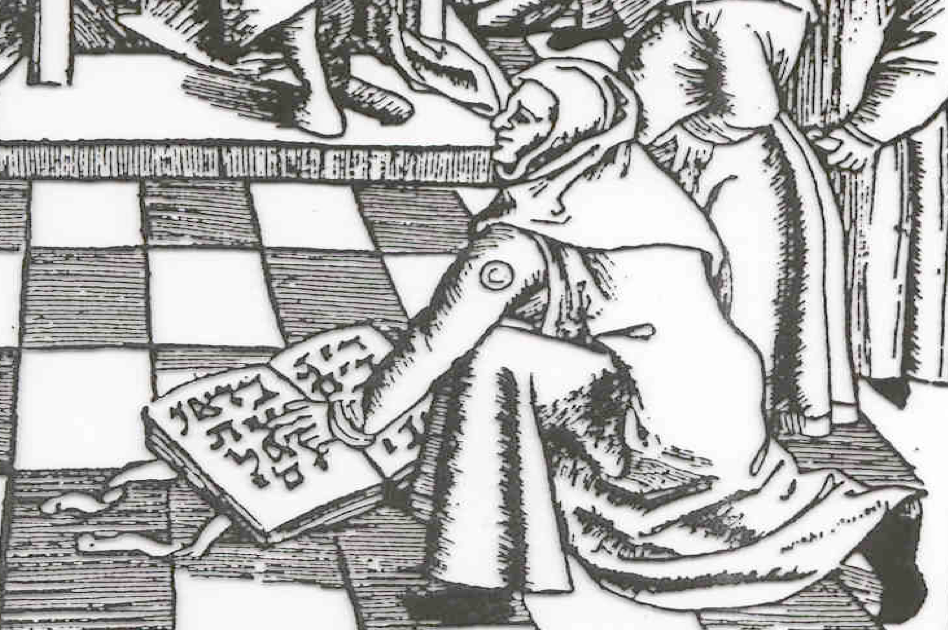
\includegraphics[width=\textwidth]{figures/judeneid_ausschnitt.png}
		\caption{\label{judeneid} Darstellung eines sog. \quein{Judeneids}: Der Schwur auf den Tanach. Ausschnitt aus einem Holzschnitt des Augsburger \qu{Laienspiegel} (1509) mit hebräischen Lettern (entnommen aus \citealt[851]{Wolf2003})} 
		\end{figure}



Es ist ein Forschungsdesiderat, die überlieferten Textzeugen und ihre Strukturen und Funktionen des \hai{{\LiHe}} zu erfassen. Bislang liegt eine Reihe von Arbeiten zu Judenfiguren in spätmittelalterlichen Schauspielen vor (\citealt{Carrington1897}; \citealt[28--29]{Lowack1905}; \citealt{Bremer1986,Frenzel1942,Frey1991,Frey1992,Frey1994,Wenzel1992,Rommel2002,Freise2002,Mikosch2010}). Allerdings geht nur \citet{Frey1992,Frey1994} näher auf die Sprache jüdischer Rollen ein.

Die Tradition des \hai{{\LiHe}} muss bis ins 17. Jahrhundert hinein ein populäres Mittel der Dramatik gewesen sein.\footnote{\cite[10]{Carrington1897} nennt als letzte Quelle Andreas Gryphius Stück \qu{Horribilicribrifax} (1663). \cite[215]{Althaus1981} findet noch im 18. Jh. Texte, die Hebraismen aufgreifen, jedoch sind dies ausschließlich sondersprachliche Quellen v.\,a.\, des Rotwelschen.} Jiddisch tritt erst ab ca.\, 1700 in die Funktion zur charakterbildenden Sprache für jüdische Rollen. Frey (\citeyear[61]{Frey1992}) findet keinerlei Anhaltspunkte für eine literarische Verarbeitung des Jiddischen in seinen Quellen des 16. Jahrhunderts (vgl.\, \citealt[24]{Frenzel1942}):

\begin{quote}
In keinem der mir bekannten mittelalterlichen Texte reden Juden, wenn sie deutsch reden, \quein{jüdelnd}. Sie reden wie ihre Antagonisten – oder aber sie reden in jener Pseudo-Sprache (die man aber als \quein{Hebräisch} ausgeben wird), die in diesem kleinen Spiel ihr absolutes Anderssein ausdrücken soll. (\citealt[61]{Frey1992})
\end{quote} 

Es finden sich tatsächlich nur wenige Hinweise auf die Verwendung jiddischer Elemente in der Figurenrede jüdischer Rollen im 16. Jahrhundert. Ein Beispiel ist Paul Rebhuns Stück \qu{Susanna} von 1536. Darin verwendet Susannas Tochter Jahel in ihrer Kindersprache das westjiddische Lexem \textit{memme} \sem{Mutter}:

 \eenumsentence{
\item \textit{We hat euch tan lieb memmelein?}\\
\sem{Wer hat euch denn lieb Mütterchen?}
\\
(Paul Rebhun \qu{Susanna} 1536: Akt 3.3; zitiert nach \citealt[29]{Lowack1905})
} 

\noindent Von diesem einen Lexem abgesehen spielt das Jiddische im Drama des 16. Jahrhunderts kaum eine Rolle (vgl.\, \citealt[28]{Lowack1905}). Dies mag mitunter an der Thematik der Stücke liegen, in denen jüdische Rollen auftreten. Als Sakralsprache der Juden ist Hebräisch für den religiösen Kontext von Passionsspielen ideal. \hai{{\LiHe}} hat keine weitere Funktion als jene, das Judentum als Gegenkonzept zum Christentum zu diffamieren (vgl.\, \citealt{Frey1992,Frey1994}). 

Am Beispiel dreier Stücke zur Laienbelehrung aus dem 16.\,Jahrhundert zeigt \cite[186]{Frey1994}, dass \hai{{\LiHe}} nur in gesonderten Gesängen Verwendung findet, nicht aber in der eigentlichen Figurenrede auftaucht, \qu{dort sprechen alle jüdischen Figuren ohne Ausnahme dasselbe Deutsch wie ihre Gegenspieler}. Damit unterscheidet sich \hai{{\LiHe}} stark vom \hai{{\LiJi}}. Der Umstand, dass jüdische Figuren im normalen Spiel wie alle anderen Figuren reden, sich aber in der Sprache ihrer Gesänge von den übrigen Figuren unterscheiden, mag soziolinguistische Verhältnisse widerspiegeln – u.\,U. war zu jener Zeit das sprachkulturelle Konzept des Jiddischen als eine nicht-deutsche Sprache längst nicht ausgebildet, worauf die Selbstbezeichnung \RL{ד{יי}\makebox(-1.5,-2.5)[r]{\libertineGlyph{uni207B}}טש}
 / \textit{daytsh} bzw. die Fremdbezeichnung als \textit{Jüdisch-Deutsch} bis ins 19. Jahrhundert hinein schließen lässt (vgl.\, \citealt{Simon1988}). Die literarische Funktion wäre demnach hinter der antisemitischen Idee verborgen, mit Hilfe des Sprachwechsels anzuzeigen, dass die Fremdartigkeit sich erst im Verborgenen zeigt. Eine solche Funktion wäre deckungsgleich mit dem Antisemitismus des 19. Jahrhunderts, wie ihn etwa Achim von Arnim vertritt (siehe dazu insbes. \citeyear[107–128]{Arnim2008}).

Die grundsätzliche Funktion des \hai{{\LiHe}} liegt grob gesprochen darin, ein negatives Gegenkonzept zum christlichen Weltbild auf die Bühne zu bringen (vgl.\, \citealt{Frey1992}). Selbst \cite[66–67]{Frey1992} räumt ein, dass das \hai{{\LiHe}} mit Laienkonzepten des Hebräischen arbeitet:

\begin{quote}
[D]as Kauderwelsch (das aber – noch – kein \quein{Jüdeln} ist, da es keiner Grammatik folgt) bedarf nicht der Übersetzung, es besteht aus Wörtern, Begriffen, Floskeln, die jeder, der ein einigermaßen scharfes Ohr hatte, beim Umgang mit Juden, beim Hören der jüdischen Liturgie in der Synagoge \quein{nebenan} aufschnappen und daher \quein{wiedererkennen} konnte. Beim gespielten \quein{Judengesang} war mithin der Fremdheitseffekt ebenso groß wie der Wiedererkennungseffekt wichtig. (\citealt[66–67]{Frey1992})
\end{quote} 

Besonders interessant ist hier, dass Frey davon ausgeht, dass das \quein{Jüdeln}, welches dem \hai{{\LiJi}} entspräche, einer \qu{Grammatik folgt}. Mit diesem Konzept vom \hai{{\LiJi}} unterscheidet er sich deutlich von den gängigen literaturwissenschaftlichen Definitionen, die \hai{{\LiJi}} auf Grundlage \,%rs auf Grundlage
von sprachlichen Regelverstößen definieren (s.\,o.). 
 
Ab 1700 findet sich kein Text mehr, der mit einem \quein{kauderwelschen} \hai{{\LiHe}} arbeitet. Doch prinzipiell bleibt Hebräisch als markierendes Element der jüdischen Figurenrede erhalten. Im \hai{{\LiJi}} spielen Hebraismen, wie zu zeigen ist (vgl.\, Kapitel \ref{hebrliji1}, S.\, \pageref{hebrliji1}), zwar eine eher untergeordnete Rolle, erhalten bleibt mit ihnen jedoch das Element, die Fremdheit der Figuren zu untermauern.


\section{Literaturjiddisch im 18. und 19. Jahrhundert}\label{literaturwissenschaft}
 
Matthias \cite{Richter1995} hat in seiner Arbeit zur \qu{Sprache jüdischer Figuren in der deutschen Literatur (1750–1933)} den Begriff des \quein{Literaturjiddischen} (\hai{{\LiJi}}) entwickelt, an dem sich auch die hier vorliegende Arbeit orientiert. Das \hai{{\LiJi}} ist ein literarisches Konzept des 18. und 19. Jahrhunderts und ein Phänomen, das zunächst auf die deutschsprachige Literatur beschränkt ist (vgl.\, Abschnitt \ref{euroliji}). Es zeichnet sich dadurch aus, dass die Literatursprache (Deutsch) im Sprechtext (direkte Rede) jüdischer Figuren formell von der nicht-jüdischer Figuren abweicht. Man findet diese literarische Strategie bei christlichen wie jüdischen Autoren (\citealt{Richter1995}).\footnote{Speziell zu jüdischen Autoren s. \cite{Gruschka2003}.} Neben \qu{als typisch jüdisch geltende[n] Namen (Itzig, Schmuel, Chohn)}, \qu{physische[n] Merkmale[n] (Nase)} oder \qu{geistige[n] oder charakterliche[n] Eigenschaften (Rechensinn, Materialismus, Feigheit)}, ist \hai{{\LiJi}} ein wesentlicher Bestandteil im literarischen Inventar zur Kennzeichnung jüdischer Figuren (\citealt[98f]{Gruschka2003}). Diese Figuren sind zumeist vom Typ des Händler- und Wucherjuden unterer sozialer Schichten.

Die Arbeiten Richters (\citeyear{Richter1995}) und Gruschkas (\citeyear{Gruschka2003}) zeigen, dass \hai{{\LiJi}} kein auf nicht-jüdische Autoren reduzierbares Phänomen ist, sondern auch von jüdischen Autoren des 19. und 20. Jahrhunderts eingesetzt wurde, nun in erster Linie, um sich als assimilierte Westjuden vom Jiddisch sprechenden Ostjudentum abzugrenzen. 

Richters Bezeichnung dieser besonderen literarischen Sprech\-eigen\-schaft als eine \quein{literarische Form des Jiddischen}, weist darauf hin, dass die jüdischen Figurenrede an die jiddische Sprache erinnert. Doch welche Eigenschaften diese fiktionale Sprache mit der natürlichen Sprache gemeinsam hat (vgl.\, Abschnitt \ref{kunstsprachen}), wird in dieser Arbeit nicht geklärt.  Wenngleich auch \cite{Richter1995} den direkten Vergleich zwischen \hai{{\LiJi}} und Jiddisch nicht scheut, hat er den Begriff des \hai{{\LiJi}} vor allem aus dem Grund eingeführt, Distanz zu schaffen zur gesprochenen Sprache, dem Jiddischen:\footnote{\citeauthor{Richter1995}s Differenzierung zwischen literarischer und gesprochener Sprache findet sich in allen Arbeiten zur Sprache jüdischer Figuren wieder (vgl.\, \citealt{FischerBayerd2008,Althaus1981,Althaus1986,Gelber1986,Glasenapp1999,Och1995,Krobb2000,Denkler1977,Gubser1998,Schreuder2002,Groezinger1998}). Einzige Ausnahme ist \citeauthor{Frenzel1942} (\citealt[105]{Frenzel1942}), die in Immermanns Stück \qu{Die Verkleidungen} (1828) den \qu{jiddischen Dialekt} wiedergegeben sieht. Den prinzipiellen Gedanken, \hai{{\LiJi}} als eine fiktionale Sprache nicht mit dem Jiddischen als eine natürliche Sprache gleichzusetzen, teilt auch diese Arbeit. Doch wie Kapitel \ref{lijisprachwissenschaft} zeigen wird, birgt der Vergleich zwischen Sprachwirklichkeit und Literatursprache ein bislang ungenutztes Potential.}

\begin{quote}
[E]s [ist] zunächst gleichgültig, ob die identifizierten Besonderheiten, die eine Figur in sprachlicher Hinsicht als jüdisch erscheinen lassen, realem Jiddisch entsprechen oder nicht. […] Es geht also weniger um Echtsein als um Echtwirken, um die Signalfunktion. Um den Unterschied zwischen tatsächlichem jüdischen Sprachgebrauch und den Sprachelementen in einer Figurenrede, die als spezifisch jüdische ausgegeben werden, nicht zu verwischen, führe ich den Begriff \quein{Literaturjiddisch} ein. Er bezeichnet die artifizielle Sprache, derer sich Autoren fiktionaler Texte zur besonderen 
sprachlichen Kennzeichnung bedienen. (\citealt[11,\,12]{Richter1995})
\end{quote}
 
Die Annahme, leicht über das \qu{Echtwirken} des \hai{{\LiJi}} entscheiden zu können, reflektiert nicht den Sitz im Leben der Texte. Es ist tatsächlich leichter herauszufinden, ob \hai{{\LiJi}} echte jiddische Formen transportiert (und damit auch ein Potenzial zum Echtwirken hat), als zu erheben, ob es auf Leser des 18. und 19. Jahrhunderts echt wirkte. Für einen Leser des 21. Jahrhunderts, der niemals im Kontakt zu einer jiddischen Varietät stand, wirken literaturjiddische Passagen tatsächlich wie fehlerhaftes Deutsch. Doch darf dies nicht auf das Lesepublikum früherer Jahrhunderte übertragen werden; dieser Fehlschluss ist leider in nahezu allen  literaturwissenschaftlichen Beiträgen zu diesem Thema zu finden. 

Trotz der postulierten strikten Trennung zwischen \ili{Westjiddisch} und \ili{Literaturjiddisch} scheut \cite{Richter1995} in seinen Analysen nicht den Vergleich zur natürlichen Sprache. Auch zeigt er anhand einiger Beispiele, dass bestimmte Reflexe der jiddischen Sprachrealität im \hai{{\LiJi}} konserviert sind (\citealt[95–113]{Richter1995}). Neben \cite{Richter1995} ist es alleine \cite{Jenzsch1974}, der zumindest in den von ihm untersuchten Dramen \qu{deutliche Spuren von Jiddisch-Imitationen} erkennt. Alle übrigen Arbeiten relativieren alle Anhaltspunkte, die auf das gesprochene Jiddisch verweisen, sehr stark und bevorzugen eine rein literaturwissenschaftliche Perspektive auf das Phänomen.

\cite[118]{FischerBayerd2008} postulieren zum Beispiel, dass sprachliche Markierungen jüdischer Figuren literarische \qu{Strategien der Sympathielenkung} sind, die \qu{von den faktualen historischen Sprechgewohnheiten abweichen}. In diesem literarischen Konzept des Jiddischen ist damit \qu{der Abgleich mit den historischen Sprachrealitäten nur von bedingtem Aussagewert} (\citealt[118]{FischerBayerd2008}). Diese Einschätzung ist in erster Linie dem mangelnden Wissen zum späten Westjiddischen geschuldet und fällt damit ein vorschnelles Urteil über den linguistischen Wert literaturjiddischer Texte. 

Viele Arbeiten, die sich der jüdischen Figurenrede nähern, verhalten sich argumentativ grenzwertig im Versuch, \textit{political correctness} zu wahren und eigene präskriptive Vorstellungen von Sprache einzupflegen. So schreibt etwa \citeauthor{Gelber1986} (\citeyear[167]{Gelber1986}) über die Figurenrede des Reb Tinkele in Gustav Freytags \qu{Soll und Haben} (1855): \qu{Die relativ leicht deformierte, syntaktisch defekte Sprache ist nur eine Andeutung seines tatsächlichen, abscheulichen Deutsch}. Entweder referiert Freytags \hai{{\LiJi}} auf das tatsächlich gesprochene, in \citeauthor{Gelber1986}s Sicht \qu{abscheuliche} Jiddisch oder aber auf ein Konzept des Lesepublikums vom Jiddischen als ein \qu{abscheuliche[s] Deutsch}. Alles in allem vertritt auch \citeauthor{Gelber1986} (\citeyear[166]{Gelber1986}) die Hypothese, dass \hai{{\LiJi}} \qu{nicht den gesellschaftlichen Verhältnissen} entspricht. Doch der Vergleichspunkt zum \hai{{\LiJi}} ist hier das Gegenwartsdeutsch Gelbers und nicht die Mündlichkeit oder die Schriftlichkeit des 19. Jahrhunderts. Dies ist der bereits erwähnte Fehlschluss, den Sitz im Leben eines Textes, also seinen historischen Kontext zu ignorieren.

Ebenso zieht Neubauer (\citeyear{Neubauer1994}) nicht das Jiddische als Vergleichssprache zum \hai{{\LiJi}} heran, sondern das moderne Standarddeutsch. 
Ein solcher Ansatz kann lediglich die Wirkung der literarischen Sprache auf die deutschsprachige Leserschaft oder das Theaterpublikum des 20. Jahrhunderts einfangen. Außer Acht gelassen wird damit der Diskurs des 19. Jahrhunderts, in dem \ili{Literaturjiddisch} nicht allein im Kontrast zum Deutschen steht, sondern vor allem im Verhältnis der Identifikation zum tatsächlich gesprochenen Jiddischen. Nur durch die Abbildung oder \isi{Imitation} der Sprachrealität in der Literatur konnte das Literaturjiddische als Identifikator jüdischer Figuren funktionieren. Neubauer (\citeyear{Neubauer1994}) möchte die Sprache ebenso zusammenphantasiert wissen, wie es bei anderen Merkmalen jüdischer Figuren (wie Inzest, Geldgier oder markante Gesichtszüge) der Fall ist. Dementsprechend charakterisiert er \hai{{\LiJi}} als eine \qu{künstliche Sprache} und \qu{nicht als natürliches Sprechen} (\citealt[144]{Neubauer1994}). Er bezeichnet phonologische und grammatische Formen als schlichtweg \qu{falsch} (\citealt[143,\,145,\,155]{Neubauer1994}) bzw. spricht sogar von \qu{linguistische[n] Fehler[n]} (\citealt[154,\,155]{Neubauer1994}), obwohl seine Beispiele Belege für charakteristisch westjiddische Formen sind.\footnote{Wie z.\,B.\, die Diphthongierungen von E2 > /ei/ und O2 > /ou/ (vgl.\, \citealt[143]{Neubauer1994}). \cite{Neubauer1994} zitiert immerhin \cite{Timm1985}, \cite{Beraneck1965} und \cite{Mieses1915}, was hieße, dass er eigentlich mehr über das Westjiddische hätte wissen können, als er vorgibt.} Selbst die Verwendung typisch westjiddischer Lexeme hat seiner Auffassung nach lediglich die Funktion, \qu{distanzierend und verfremdend} auf das Publikum zu wirken (\citealt[142]{Neubauer1994}), als dass sie auf eine literaturexterne Sprachrealität verweisen könnten. 

Doch die Frage, ob \hai{{\LiJi}} die jiddische Sprachrealität abbildet, mag für das nicht Jiddisch sprechende Lesepublikum keine Relevanz gehabt haben. Viel entscheidender ist jedoch, ob \hai{{\LiJi}} den Erwartungen und Konzepten des Jiddischen entspricht. Dies lässt sich jetzt kaum mehr feststellen. So kommt \cite{Gubser1998} zu dem Schluss, das \hai{{\LiJi}} sei \qu{für die deutschsprachige Mehrheit zweifelsohne nur schwer zu verstehen} gewesen. Dieses \quein{Nichtverstehen} ist laut Gubser (\citeyear[138f]{Gubser1998}) das zentrale Element jüdischer Figuren. Ein besonders eindrucksvolles, \citeauthor{Gubser1998}s Idee widersprechendes Beispiel liegt im Fall eines 1739 verfassten Hochzeitsgedichts eines Herrn Arletius aus Breslau vor. Der Verfasser gibt selbst an, \qu{daß die Kenner des Jüdischen [= Jiddischen, L.S.] es durchaus nicht für das Werk eines nicht jüdischen Verfassers halten wollen} (\citealt[281]{Arletius1800}). Diese Beurteilung lässt zwei Schlüsse zu: Entweder hatte das nicht-jüdische Publikum nur eine sehr begrenzte Vorstellung vom tatsächlich gesprochenen Jiddisch, dass es ausreichte, ein \quein{verfremdetes Deutsch} einzusetzen, oder aber die \isi{Imitation} entspricht derart stark einem aus dem direkten \isi{Sprachkontakt} resultierendem Konzept des Jiddischen, was dafür spricht, im \hai{{\LiJi}} Reflexe aus der Sprachrealität zu vermuten.

Obzwar kaum eine der Arbeiten, die sich mit der Sprache jüdischer Figuren befassen, sprachwissenschaftliche Analysewerkzeuge verwendet gibt es doch Bestrebungen, die Besonderheiten des \hai{{\LiJi}} einzufangen. Die am häufigsten genannten sprachlichen Markierungen jüdischer Figurenrede, die sich in der aktuellen Forschungsliteratur finden lassen, sind die folgenden:

\newpage 

\begin{itemize}

\item [–] \textbf{Extrapositionen  (Nachfeldbesetzung)} \qu{Eigentümlichkeiten der Wortstellung} (\citealt[104]{Richter1995}), \qu{Umstellungen und Ausklammerungen} (\citealt[219]{Althaus1981}), \qu{Endstellung des Akkusativ-Objektes […] aber auch adverbiale[r] Bestimmungen und andere[r] Objekte}  (\citealt[187]{Jenzsch1974}), z.\,B.\, \textbf{NP-Extraposition} \textit{zu machen ein groß Geschäft} \sem{um ein großes Geschäft zu machen} (Felix Dahn \qu{Ein Kampf um Rom} (1876), zit.\,n. \citealt[104]{Richter1995}); \textbf{PP-Extraposition} \textit{wenn der Herr Ehrenthal, für mich nicht hat ein Bett in seinem Hause} \sem{wenn der Herr Ehrenthal für mich nicht ein Bett in seinem Hause hat} (Gustav Freytag \qu{Soll und Haben} [im Folgenden \hai{SH} (Kluczbork, 1855)], zit.\,n. \citealt[220]{Althaus1981}); \textbf{AP-Extraposition} \textit{So laß mich nicht reden umsonst} \sem{lass mich nicht umsonst reden} (Felix Dahn \qu{Ein Kampf um Rom} (1876), zit.\,n. \citealt[104]{Richter1995})\label{bspform1} 
	
\item [–] \textbf{symmetrisches-V2} \qu{nicht-finale Stellung der finalen Stellung im Gliedsatz} (\citealt[100]{Richter1995}), \qu{Aufhebung der Klammerstellung des Verbs am Satzende der Nebensätze} (\citealt[219]{Althaus1981}), \qu{fehlerhafte, dem Hauptsatz-Ge\-fü\-ge nachempfundene Setzung des Prädikats an zweiter Stelle im Nebensatz} (\citealt[141]{Gubser1998}), \qu{stereotype Aufhebung der Klammerstellung des Verbs} (\citealt[143]{Neubauer1994}) z.\,B.\, […] \textit{brauchste dich nicht lassen zu treten} (Wilhelm Raabe \qu{Der Hungerpastor} (1864), zit.\,n. \citealt[100]{Richter1995})\label{bspform2} 

\item [–] \textbf{verb raising} \qu{die unmittelbare Nachsetzung des Partizips Perfekt hinter das Hilfsverb im Hauptsatz} (\citealt[141]{Gubser1998}), \qu{fehlerhafte Stellung des Prädikats in Nebensätzen} (\citealt[141]{Gubser1998}), z.\,B.\, \textit{das schaine Geld, was er hat mitgenommen} \sem{das schöne Geld, welches er mitgenommen hat} (Karl Borromäus Sessa \qu{Unser Verkehr} (1816), zit.\,n. \citealt[141]{Gubser1998})\label{bspform1b} 
	
	\item [–] \textbf{Kasus nach Präposition} \qu{[Gebrauch] des Akkusativs anstelle des Dativs}  (\citealt[102]{Richter1995}), z.\,B.\, \textit{Leute von den juten Ton} \sem{Leute von gutem Ton} (Wilhelm Hauff \qu{Mitteilungen aus den Memoiren des Satan} (1825/26), zit.\,n. \citealt[102]{Richter1995})\label{bspform4a} \textbf{Kasussynkretismen bei Personalpronomen} \qu{Gebrauch des Dativs anstelle des Akkusativs} (\citealt[102]{Richter1995}), z.\,B.\, \textit{hat mir gekostet} \sem{hat mich gekostet} (Wilhelm Hauff \qu{Mitteilungen aus den Memoiren des Satan} (1825/26), zit.\,n. \citealt[102]{Richter1995})\label{bspform4b} 
	
	
	\item [–] \textbf{Adjektivflexion} \qu{unflektierte[s] \isi{Adjektiv} in attributiver Stellung} (\citealt[104]{Richter1995}), z.\,B.\, \textit{zu machen ein groß Geschäft} \sem{um ein großes Geschäft zu machen} (Felix Dahn \qu{Ein Kampf um Rom} (1876), zit.\,n. \citealt[104]{Richter1995})\label{bspform1q} 
	  
\newpage 
	\item [–] \textbf{Klitisierungen} \qu{kontrahierte Form} (\citealt[101]{Richter1995}), z.\,B.\, \textit{gebts} \sem{gebt es}  (s. \citealt[225 ]{Althaus1981}) oder \textit{kannste} \sem{kannst du} (Wilhelm Raabe \qu{Der Hungerpastor} (1864), zit.\,n. \citealt[100]{Richter1995})\label{bspform3} 
	
	%\item [–] \textbf{Auslautverhärtung} \qu{die Verhärtung ch, g > k am Wortende}  (\citealt[177]{Jenzsch1974}), z.\,B.\, \textit{Heinrick} \sem{Heinrich}  (\citealt[177]{Jenzsch1974})\label{bspform3q} 

	
		\item [–] \textbf{-t/-d Ellision} \qu{Abschleifung der Konsonanten} (\citealt[143]{Neubauer1994}), z.\,B.\, \textit{unn} \sem{und} (\citealt[143]{Neubauer1994})\label{bspform9} 

\item [–] \textbf{Mhd. \textit{ou}, \textit{ei} > /a\textlengthmark/}\qu{lautliche Besonderheiten des Jiddischen} (\citealt[217]{Althaus1981}), \qu{Monophthongierung} (\citealt[143]{Neubauer1994}), z.\,B.\, \textit{ka} \sem{kein}, \textit{Ag}, \sem{Auge} (Maler Müller \qu{Fausts Leben dramatisiert} (\hai{FL}), zit.\,n. \citealt[217]{Althaus1981}); es findet sich aber aber auch die Feststellung \qu{steht für nhd. \sem{ei} = jidd. \sem{ee, ä}} \textit{keen} \sem{kein}  (\citealt[177]{Jenzsch1974})\label{bspform6} 
	
	
	\item [–] \textbf{Mhd.\textit{ê} > /ei/} \qu{Diphthongierung} (\citealt[143]{Neubauer1994}),  z.\,B.\, \textit{gaiht} \sem{geht} (\citealt[143]{Neubauer1994})\label{bspform7} 
	
	\item [–] \textbf{Mhd. \textit{ô} > /ou/}  \qu{Diphthongierung} (\citealt[143]{Neubauer1994}), z.\,B.\, \textit{wouhl} \sem{wohl} (\citealt[143]{Neubauer1994})	\label{bspform8} 

		\item [–] \textbf{/a/, /a\textlengthmark/ > /o/, /o\textlengthmark/ (\isi{a-Verdumpfung})} \qu{statt nhd. \sem{a} findet sich jid. \sem{o}} z.\,B.\, \textit{Johr} \sem{Jahr} (\citealt[177]{Jenzsch1974}).\label{bspform10} 

	
	\item [–] \textbf{Jiddismen, Hebraismen und (fehlerhafte) Fremdwörter} z.\,B.\, \textit{Bonem} \sem{Gesicht} (s. \citealt[217]{Althaus1981}); \textit{Rosch} \sem{Kopf} (s. \citealt[217]{Althaus1981}); \textit{Perzent} \sem{Prozent} (s. \citealt[108f,\,115–122]{Richter1995}; s.\,a. \citealt[142]{Neubauer1994})\label{bspform4} 
		
	\item [–]  \textbf{Psychoostentative Ausdrücke} \qu{\textit{typisch} jüdische Interjektionen}  (\citealt[141]{Gubser1998}) z.\,B.\, \textit{Nu!} \sem{Nun}, \textit{Au weih!} \sem{Oh weh!} (Jakob Grimm \& Wilhelm Grimm \qu{Der Jud' im Dorn} (1812), Georg Büchner \qu{Woyzeck} (1836/37) zit.\,n. \citealt[142]{Gubser1998})\label{bspform5} 
	
\end{itemize}

Allen Arbeiten liegt eine Scheu zugrunde, \ili{Literaturjiddisch} mit gesprochener Sprache in direkte Beziehung zu setzen; besonders deutlich formuliert dies Richter:

\begin{quote}
Festzuhalten bleibt jedoch, dass auch wenn ein Merkmal noch so oft in fiktionalen Texten vorkommt, es zunächst doch immer als ein Merkmal des Literaturjiddischen aufzufassen ist. Auch hochgradige Merkmalsrekurrenz sollte nicht dazu verleiten, die Trennung von Fiktion und Realität zu verwischen. Diese Trennung strikt zu beachten, ist aber ganz besonders im Hinblick auf die Geschichte der Juden in Deutschland angezeigt, wo Wissen oft auf verheerende Weise mit dem bloßen Meinen und Wähnen, mit Vorurteilen, Mythen und Legenden über die Juden verquickt war. (\citealt[99]{Richter1995})
\end{quote}

\noindent Entgegen Richters (\citeyear[99]{Richter1995}) Appell werden in der vorliegenden Arbeit die literaturjiddischen Merkmale zum Zweck einer linguistischen Auswertung ihrer literarischen Funktion enthoben und in der Analyse der Teilphänomene \textbf{wie} Daten natürlicher Sprache behandelt, denn nur so können Vorurteile, Mythen oder Ideen überprüft werden.\, %Wie die Analyse dieser Arbeit zeigt (Abschnitt \ref{analysen}), verweisen beinahe alle der hier genannten Phänomene auf das tatsächlich gesprochene Jiddische. 
Ohne eine solche Detailanalyse ist es schwer zu entscheiden, ob das \hai{{\LiJi}} des 19. Jahrhunderts auf Formen des Westjiddischen zurückgreift oder auf Formen des Ostjiddischen, welches besonders im Verlauf des 19. Jahrhunderts aufgrund von Migrationsbewegungen auch im deutschsprachigen Raum (insbes. in Großstädten) durchaus als Kontaktsprache zum Deutschen gegeben ist (vgl.\, \citealt{Bertram1924,AdlerRudel1959,Maurer1986}; \citealt[229–239]{Gay1994}).\label{RueckgangWJimLiJi} Diese Arbeit geht davon aus, dass bis in die zweite Hälfte des 19. Jahrhunderts \ili{Westjiddisch} als noch durchaus vitale Sprache im deutschsprachigen \,%rs -n
Raum verbreitet war und der ostjiddische Einfluss noch als marginal zu erachten ist. Für das Literaturjiddische ab 1850 hingegen nehme ich – aufgrund des einsetzenden westjiddischen Sprachtods und der zunehmenden Einwanderung von Sprechern des Ostjiddischen ab den 1880er Jahren (vgl.\, \citealt[229–239]{Gay1994}) – vorläufig einen Anstieg \ili{ostjiddisch} beeinflusster Strukturen an. Doch erst die Detailanalyse kann diese Hypothese bestätigen.

 In erster Linie arbeitet \ili{Literaturjiddisch} mit dem Kontrast von gesprochener vs. geschriebener Sprache. Dies wird besonders mit Blick auf die zahlreichen Theaterstücke des 19. Jahrhunderts deutlich: Jüdische Figuren werden anhand ihrer Sprache symbolisch aus dem Kulturkreis des Schriftdeutschen ausgeschlossen. Von der Konzeption her sind jedoch alle dramatis personae an der Mündlichkeit orientiert (vgl.\, \citealt{KochOesterreicher1985}). Im Gegensatz zu allen anderen Figuren zeichnen sich aber nur die jüdischen Figuren durch eine Nähe zur gesprochenen Sprache aus. Auf welches sprachliche Wissen der jeweilige Autor des Literaturjiddischen zurückgreift, wenn er diese Dialektalität auf die Bühne bringen will, ist nicht klar zu bestimmen. Neben dem Jiddischen können Strukturen des Literaturjiddischen im 19. Jahrhundert aber auch durch Dialektkompetenz des Autors oder auch durch Konzepte anderer deutscher Varietäten beeinflusst worden sein. Aber auch durch Sprachpolitik und Sprachpurismus als pejorativ verurteilte Strukturen können dazu eingesetzt werden, den Sprecher einer solchen Struktur herabzusetzen.  All diese möglichen Einflüsse müssen bei der Analyse literaturjiddischer Strukturen berücksichtigt werden.
 
  
Es liegen keine direkt vergleichbaren sprachwissenschaftlichen Analysen zur Verwendung deutscher Umgangssprache oder Dialekte in der Literatur des 19. Jahrhunderts vor. Aus der Leseerfahrung literaturjiddischer Texte kann ich lediglich darauf verweisen, dass in den Texten, in denen \hai{{\LiJi}} auftritt, hochdeutsche Dialekte keine Rolle spielen. Eine Ausnahme stellen niederdeutsche Texte dar, in denen die Matrixsprache an sich ein Dialekt ohne Schreibnorm ist. Eine dramatische Verarbeitung gesprochener Sprache jenseits des \hai{{\LiJi}} setzt in der Literatur \,%rs des zuviel
erst gegen Ende des 19. Jahrhunderts ein. Besonders im Theater des Naturalismus tritt mehr und mehr gesprochene Sprache im deutschen Drama auf, wie z.\,B.\, in Gerhart Hauptmanns Stück \qu{Vor Sonnenaufgang} (1889), in welchem dem schlesischen Dialekt eine besondere dramaturgische Rolle zukommt. Außerhalb des Dramas erhält gesprochene, dialektale Sprache v.\,a.\, im niederdeutschen Raum einen besonderen Stellenwert. Wiederum sind hier naturalistische Werke wie die  Theodor Fontanes (1819–1898), Fritz Reuters (1810–1874) oder Theodor Storms (1817–1888) zu nennen. Angelika Linke (\citeyear[231--264]{Linke1996}) zeigt auf, dass Dialektalität im Bürgertum des 19. Jahrhunderts durchaus als Kontrastelement zur angestrebten Standardsprachlichkeit eine wichtige Rolle spielte. In der Literatur trägt die Verwendung von Dialekt laut Mattheier (\citeyear{Mattheier1993}) und Linke (\citeyear[239f]{Linke1996}) generell zwei Funktionen: Dialekt dient dazu, Komik und/oder Realitätsnähe zu evozieren. Damit würde sich die literarische Verwendung des Jiddischen rein qualitativ kaum von der deutscher Dialekte unterscheiden. Rein quantitativ überwiegen jedoch die Fälle, in denen die jiddische Sprache zu diesen Zwecken eingesetzt wird.  Kein deutscher Dialekt ist in der deutschsprachigen Literatur dermaßen präsent, wie wir es im Fall des Jiddischen anhand der jiddischen Imitationen sehen. 


\section{Sprachliche Markierungen des assimilierten Juden}\label{assimiliert}
 
In der Literatur des 19. Jahrhunderts finden sich neben dem Literaturjiddischen weitere Stilmittel, jüdische Figuren über ihre Sprache zu charakterisieren. Diese dienen besonders dazu, den Typus des assimilierten Juden der bürgerlichen Oberschicht  als einen solchen erkennbar zu machen. Da in dieser Bevölkerungsschicht das Jiddische keine Rolle mehr spielt, müssen andere Strategien zur Figurenbildung eingesetzt werden. 
 
  Eine dieser Strategien ist das sogenannte \quein{Überdeutsch} (\citealt[174–175]{Gelber1986}). Diese sprachliche Besonderheit findet sich laut Gelber (\citeyear[174–175]{Gelber1986}) etwa in Thomas Manns \qu{Doktor Faustus} (1947) in den Figuren Dr. Chaim Breisacher und Kunigunde Rosenstiel. Das Konzept vom \quein{Überdeutschen} tritt jedoch nur selten in der Literatur des 19. Jahrhunderts auf. Ein Beispiel ist der nachfolgende Ausschnitt aus dem stark antisemitisch geprägten Stück \qu{Unser Verkehr} des Breslauer Augenarztes Karl B.\,Sessa. \quein{Überdeutsch} wirkt hier besonders durch den Kontrast zwischen dem Literaturjiddischen des als geistig minderbemittelt dargestellten Jakobs und dem  überzeichneten Schriftdeutsch (\quein{Überdeutsch}) des studierten Juden Isodorus Morgenländer (vgl.\, \citealt[174–175]{Gelber1986}).\footnote{Doch selbst in der Figurenrede des Isodorus lassen sich Relikte des \hai{{\LiJi}} finden: Wie alle anderen jüdischen Figuren des Stückes verwendet auch er Extrapositionen von \hai{PP}s wie z.\,B.\, \textit{Ich bin gereist auf Akademien und Universitäten}, \textit{ich bin gewesen in Jena und Halle, […]}; Allerdings könnte hier auch u.\,U. Behagels \quein{Gesetz  der Wachsenden Glieder} wirksam sein, nach dem \quein{schwere Phrasen} leichter extraponiert werden können als \quein{leichte} (vgl.\, \citealt{Behaghel1909}; s. auch Kapitel \ref{VOOV}, S.\, \pageref{VOOV}).} Im \quein{Überdeutschen} funktioniert die sprachliche Karikatur komplementär zum Literaturjiddischen: Das dargestellte Unvermögen, \quein{korrektes Deutsch} zu sprechen, wird hier mittels überkorrektem Deutsch auf die Bühne gebracht.  

%\begin{quote}
\begin{itemize}
\begin{footnotesize}
\begin{itshape}
\item[Jakob.] Du host getrunken? Host de getrunken ä Schnaps? – Du host doch genummen ßu viel!
\item[Isidorus.] Vernimm! – Ein mysthisch Dunkel ruht auf dem Jahre meiner Abwesenheit.
\item[Jakob.] Jo, ä Johr bist du gewesen weg.
\item[Isidorus.] Ihr Alle wisst nicht: wie? wo? wann?
\item[Jakob.] Mer hoben gedacht, du wärst uf en Handel?
\item[Isidorus.] Höre meine Geschichte! – – Unter den Ochsen meines Vaters ward ich auferzogen, und lebte ein stilles nomadisches Leben, wie die ersten Menschen im Stande der Unschuld, \so{objectiv}, und von der Natur noch nicht getrennt. Aber, wie in jenen Chaldäern und Hebräern, unsern Urvätern, in ihrer Beschauung eine Ahnung des Höchsten erwachte – so in mir! – Ich verließ meine Ochsen und suchte die Weisheit. 
\item[Jakob.] De Weisheit?
\item[Isidorus.] Ich bin gereist auf Akademien und Universitäten; ich bin gewesen in Jena und Halle, in Marburg und Würzburg, in Bamberg und Heidelberg, in Königsberg und Wittenberg, in Leipzig und Helmstädt, in Tübingen und Göttingen, in Breslau und Krakau, in Padua und Pavia.
\item[Jakob.] (schlägt die Hände verwundert zusammen.) Du bist geworden ä Dokter?
\end{itshape}
\item[] (Sessa \qu{Unser Verkehr}; Breslau [1810]1816:\,50–52)
\end{footnotesize}
%\end{quote}
\end{itemize}

Das Konzept vom \quein{Überdeutschen} ist nicht zu verwechseln mit Hyperkorrekturen bzw. Übergeneralisierungen, etwa von Fremd- und Lehnwörtern oder dem gesprochenen Deutsch, wie sie z.\,B.\, in Episoden auftreten, in denen eine jüdische Figur versucht, ihre (literatur-)\,jiddischen Sprachgewohnheiten abzulegen. Ein Beispiel für solche Strategien findet sich in Passagen der Rede des \textit{Veitel Itzigs} in Gustav Freytags Roman \qu{Soll und Haben} (1955), wenn diese Figur versucht, ihr sonstiges (Literatur-)Jiddisch zu vermeiden.

Ein mit dem \quein{Überdeutsch} eng verwandtes sprachliches Stilmittel ist das sogenannte \quein{Juden-Französisch-Deutsch} (\citealt[175]{Gelber1986}),\label{judenfranzoesischdeutscherstmals} welches mittels Gallizismen ein \quein{fehl}-assimiliertes (West-)Judentum charakterisieren will. Beispiele hierfür finden sich im Analyseteil in Abschnitt \ref{galliliji1} (S.\, \pageref{galliliji1}). Hinter dieser sprachlichen Markierung jüdischer Figuren steckt die Symbiose zweier Feindbilder: Antisemitismus und Franzosenhass gehen seit der französischen Revolution und insbesondere den napoleonischen Kriegen im Deutschland des 19. Jahrhunderts einher (vgl.\, \citealt[18, 68–70]{Gubser1998}; \citealt[139–149]{Hartung2006}). Damit ist jeder \isi{Gallizismus} im Mund einer jüdischen Figur auch als ein \textit{Lippenbekenntnis} zu verstehen, mit den \textit{französischen Feinden} zu kooperieren. Wie der Anti-Napoleonismus reicht das \quein{Juden-Französisch-Deutsch} über das 19. Jahrhundert hinaus und findet sich bis weit ins 20. Jahrhundert hinein. Hier sei wiederum auf Manns \qu{Doktor Faustus} verwiesen, wo in der Sprache des Juden \textit{Saul Fitelbergs} überdurchschnittlich viele Gallizismen und französische Phrasen zu finden sind (vgl.\, auch \citealt[142]{Hartung2006}).

Der tendenziös antisemitische Autor Karl Theodor Griesinger schreibt in seiner Charakterisierung von assimilierten Juden: \qu{Der aufgeklärte Jude zählt unter seinen Mitgliedern blos Männer, er spricht deutsch und französisch} (\citealt[222]{Griesinger1838}). Man greift also auch bei jüdischen Figuren, die sich aller als charakteristisch \quein{jüdisch} geltender Merkmale entledigt haben, weiterhin, trotz sprachlicher \isi{Assimilation}, auf eine Kennzeichnung jüdischer Figuren mittels sprachlicher Abweichungen von der Schriftsprache zurück, wie man es aus dem Literaturhebräischen und  Literaturjiddischen kennt. 



\section{Literaturjiddisch nach 1945} 
 
Der Diskurs um das Jiddische in der deutschsprachigen Literatur bricht nach 1945 nicht ab. \ili{Literaturjiddisch} erlangt zwar nicht wieder einen solchen Aufschwung wie im 19. Jahrhundert, bleibt aber im kollektiven Gedächtnis der Literatur- und Kulturschaffenden und findet so auch immer wieder vereinzelt Einzug in die Nachkriegsliteratur. Max Frischs Theaterstück \qu{Als der Krieg zu Ende war} (1948) (\hai{AK})\footnote{Obwohl dieser Text rein zeitlich nicht mehr dem Stadium des \hai{{\LiJieins}} zuzurechnen ist, wurde er als Endpunkt in das Untersuchungskorpus zum \hai{chrLiJi1} aufgenommen um einen Einblick in die Kurzzeitdiachronie des \hai{{\LiJieins}} gewinnen zu können.} oder Paul Celans \qu{Gespräch im Gebirg} (1959) können als erste Wiederaufnahme des \hai{{\LiJieins}} nach 1945 gelten. In letzterem dient die Dekonstruktion der Sprache selbstverständlich nicht allein der \isi{Imitation} des Jiddischen. Bei genauerer Analyse fällt jedoch auf, dass Celan sich hier eben jener aus dem \hai{{\LiJieins}} bekannten (vorwiegend syntaktischen) Manipulationen bedient. 

Die Sprache jüdischer Figuren in der Literatur nach 1945 wurde bislang nicht näher untersucht. Die im Vergleich zum 19. Jahrhundert wenigen Arbeiten zu Judenfiguren der Nachkriegs- und Gegenwartsliteratur geben keine Anhaltspunkte, dass eine Fortsetzung der Verwendung des \hai{{\LiJi}} im 20. und 21. Jahrhundert stattfand (vgl.\, \citealt{Heuser2011,Mueller1984,Schmelzkopf1983}). Eine exemplarische Durchsicht von Texten mit jüdischen Figuren hat jedoch ergeben, dass seit den 1980er Jahren und besonders seit der Jahrtausendwende ein Anstieg von Texten zu verzeichnen ist, die sich eine sprachliche Markierung zu Nutze machen. Um nur eine Auswahl an Texten zu nennen, findet sich \hai{{\LiJi}} in André Kaminskis \qu{Nächstes Jahr in Jerusalem} (1986), Rafael Seligmanns \qu{Der Milchmann} (1999) oder in der deutschen Übersetzung von Noah Gordons \qu{The Physician} (1986) [\qu{Der Medicus} (1986)]. 
Vorzugsweise findet sich dieses Phänomen in der Prosa und wird besonders in Übersetzungen aus dem Englischen ins Deutsche eingesetzt. Wie die Analysen einer kleinen Auswahl moderner Texte in \textcite{SchaeferDiss} zeigt, orientiert sich das moderne \hai{{\LiJizwei}} stärker am Ostjiddischen. Bemerkenswert ist, dass \hai{{\LiJizwei}} nun seine pejorative Funktion (vgl.\, Abschnitt \ref{Kapitel Funktionstypen}) gänzlich verloren zu haben scheint und nur mehr rein charakterbildend für einen jüdisch-orthodoxen Figurentyp mit osteuropäischen Wurzeln ist. Dem entspricht auch die Feststellung, dass \hai{{\LiJizwei}} nur von Autoren mit jüdischem Hintergrund verwendet wird (bzw. von Übersetzern jüdischer Autoren). Als Texte mit literaturjiddischen Elementen, die das Westjiddische als Zielsprache haben, können lediglich der historische Roman \qu{Melnitz} (2006) von \ia{Lewinsky, Charles}
sowie einzelne Erzählungen des Badischen Autors \ia{Picard, Jacob} (1883–1967) genannt werden.    


\section{Die Sprache jüdischer Figuren im Film}\label{fiji}

Sprache als identitätsstiftendes Merkmal ist immer ein Element von Theater und Film. Eine dramatische Rolle wird mittels idiosynkratischer, dialektaler oder soziolektaler sprachlicher Auffälligkeiten entworfen. Der Film der Gegenwart ist voller sprachlicher Stereotype (Medialekte): von einer aus Louisiana stammenden Figur wird der Akzent der Südstaaten (Southern American English) erwartet (wie etwa in der Serie \qu{True Blood}, 2008--2014); Rollen lateinamerikanischer Stereotype sind über spanische oder portugiesische Kennwörter oder Phrasen identifizierbar (z.\,B.\, in der Serie \qu{Dexter}, 2006--2013); auch werden idiosynkratische Eigenschaften historischer Personen nachgeahmt, wie etwa die von Truman Capote im Fim \qu{Capote} (2005). So verwundert es nicht, dass auch jüdische Figuren im Film sprachlich gekennzeichnet werden. Im Unterschied zu englischen Soziolekten und Dialekten können sprachliche Markierungen, die auf dem Jiddischen basieren, bei Synchronisationen vom Englischen ins Deutsche übertragen werden; nicht zuletzt, weil im deutschsprachigen Raum bereits eine Tradition jüdischer Figurenrede vorliegt, an die angeknüpft werden kann. Auch in deutschsprachigen Produktionen sind medienwirksame Aufbereitungen deutscher Dialekte Usus, wie etwa das sogenannte \quein{Medienbairisch} (vgl.\, \citealt{Kleiner2013,Riemann2009,MayerZimmerer2009}). Distanzmessungen zwischen Oralisierungsnorm, Basisdialekt und Medien\ili{bairisch} zeigen, dass nur ein kleines Repertoire phonologischer Markierungen, die zumeist lexemgebunden sind, nötig sind, um Bairisch im deutschsprachigen Film anzudeuten (\citealt{Kleiner2013,Riemann2009,MayerZimmerer2009}). Interessante Ergebnisse kann hier ein Vergleich zwischen den Strukturen solcher Mediendialekte und dem \ili{Filmjiddisch} liefern.

Das Aufkommen des \hai{{\LiJizwei}} im 20. Jahrhundert ist m.\,E. eng an Entwicklungen der jüdischen Figurensprache im Film geknüpft, vielleicht sogar durch diese inspiriert. Seit den 1980ern mehren sich Filme, in denen sich die Sprache jüdischer Figuren von der übriger Charaktere unterscheidet bzw. Jiddismen eine besondere Rolle der Figurencharakterisierung einnehmen. Ich nenne dieses Phänomen \ili{Filmjiddisch} (\hai{{\FiJi}}). Es betrifft vor allem, aber nicht ausschließlich, englischsprachige, insbesondere amerikanische Produktionen.\footnote{Filme bzw. Serien, in denen sich \hai{{\FiJi}} findet, sind z.\,B.\, \qu{Some Like It Hot} (dt. \qu{Manche mögen’s heiß}) (1959), \qu{An American Tail} (dt. \qu{Feivel der Mauswanderer}) (1986), \qu{Snatch} (dt. \qu{Schweine und Diamanten}) (2000), \qu{Ocean’s Twelve} (dt. \qu{Ocean’s 12}) (2004), \qu{Alles auf Zucker} (2004), \qu{The Infidel} (dt. \qu{Alles Koscher}) (2010), \qu{The Dictator} (2012), \qu{The Simpsons} (1987–), \qu{Futurama} (1998–2003, 2007–2013), \qu{Family Guy} (1999–), \qu{Seinfeld} (1989–1998), \qu{South Park} (1997–),\qu{The Nanny} (1993–1999), \qu{The Sopranos} (1999–2007), \qu{The Big Bang Theory} (2007–), \qu{Boardwalk Empire} (2010–2014), \qu{Broad City} (2014– ), \qu{Transparent} (2014–). Einen Sonderfall stellt der Film \qu{A Serious Man} (2009) von Ethan und Joel Coen dar. Diesem Film ist ein jiddischer Prolog vorangestellt, der in allen Synchronfassungen erhalten, d.\,h. untertitelt wurde. Hier lässt sich weniger von \textit{Filmjiddisch} als eher von einem jiddischen (Kurz-)Film sprechen.} \hai{{\FiJi}} findet besonders in amerikanischen Fernsehserien Verwendung und wird weniger in Spielfilmen gebraucht. Hier finden sich Tendenzen, das moderne Ostjiddische bzw. das daraus hervorgegangene \textit{Jewish-English} (vgl.\, u.\,a.\, \citealt{Fishman1985,Gold1985,Benor2009}) zu imitieren. Formen des ausgestorbenen \ili{Westjiddisch} spielen selbstverständlich keine Rolle.

In der Medienwissenschaft wurde diese jüngere Entwicklung bislang in nur wenigen Randnotizen gewürdigt. \cite[129]{Bothe2013} und \cite[383]{Zeifert2013} finden in den von ihnen analysierten Filmen das \qu{Jiddische} wieder. \cite[90]{Haselberg2013} beurteilt differenzierter die Sprache einer jüdischen Figur als \qu{besonders in der Satzstellung, von einem Akzent gefärbt, der jiddisch anmutet}. \cite[78]{Lubrich2008} geht in seiner Analyse von Dani Levys \qu{Alles auf Zucker} (2004) in einem kurzen Abschnitt auf die Sprache als charakterbildendes Element ein. Er beschreibt die Sprache als \qu{osteuropäische[n] Akzent}, \qu{jiddische[n] Dialekt} mit der starken Verwendung von Hebraismen und kommt zu dem Schluss, dass dies \qu{alles andere als normales Hochdeutsch} sei (\citealt[78]{Lubrich2008}).


Die Sprache jüdischer Figuren im Film näher zu untersuchen, wäre wiederum eine eigene Forschungsarbeit wert. Besonders interessant ist der Vergleich verschiedener Synchronisationen. \hai{{\FiJi}} findet sich verstärkt in deutsch- und englischsprachigen Filmen. In z.\,B.\, \ili{französisch}- oder italienischsprachigen Filmen sind keine bis wenige sprachliche Auffälligkeiten jüdischer Figuren zu erkennen. Ein gutes Beispiel sind hierfür die verschiedenen Synchronisationen von Mihăileanus \qu{Train de vie} (dt. \qu{Zug des Lebens}) (1998). Der im Original französischsprachige Film, der die phantastische Geschichte eines osteuropäischen Shtetls erzählt, arbeitet, abgesehen von sehr wenigen hebräischstämmigen Wörtern (\ref{bspfiji1}), mit keinerlei sprachlichen Markierungen, obwohl er inhaltlich die jiddische Sprache mehrmals thematisiert (insbes. 17.00–17.25\,min). Und auch die italienische Synchronisierung benutzt wie das Original lediglich vereinzelt lexikalische Elemente (\ref{bspfiji1b}),\footnote{Filmbelege werden im Folgenden nach der \isi{Orthographie} der Matrixsprache wiedergegeben; Jiddismen folgen den Richtlinien des YIVO. Eine phonetische Wiedergabe wäre im Zuge detaillierter Analysen sinnvoll.} um auf das Jiddische zu verweisen.

\eenumsentence{
	\item \textit{il est meshuge} \sem{er ist verrückt} (\textit{Train de vie} [OV] 1998:\,19.37\,Minute)
	\label{bspfiji1} 

	\item \textit{lui è meshigo} (\textit{Un treno per vivere} 1998:\,19.37\,Minute)
	\label{bspfiji1b} 

	\item \textit{er is meshige} (\textit{Zug des Lebens} 1998:\,19.53\,Minute)
	\label{bspfiji2} 
}

\noindent Die deutsche Synchronisierung des Films arbeitet hingegen viel mit diversen prosodischen, phonologischen und morphosyntaktischen Markierungen in der jüdischen Figurenrede. Die jüdische Figurenrede wurde in der deutschen Synchronisation systematisch von der Originalsprache des Films abweichend konstruiert. So findet man z.\,B.\, die \isi{Entrundung} /y/ > /i/ (\ref{bspfiji5}), der stimmlose palatale \isi{Frikativ} wird als stimmloser velarer \isi{Frikativ} realisiert (/ç/ > /x/) (\ref{bspfiji6}), der Vokal \hai{V44} (\hai{O4} = {\mhd} \textit{ou}) wird als /\textopeno \textsubarch{\textsci}/ (\ref{bspfiji7}) und der Vokal \hai{V22} (\hai{E2} = {\mhd} \textit{ê}, \textit{œ}) als /aɪ̯/ (\ref{bspfiji8b}) wiedergegeben.\footnote{Zur Notation des protojiddischen Vokalsystems siehe Abschnitt \ref{phonologie}, S.\, \pageref{phonologie}.} %Syntaktische Auffälligkeiten treten hinter phonologisch-phonetische. 
Auffällig sind etwa der Verzicht auf den \isi{Ersatzinfinitiv} (\hai{No-IPP}) (\ref{bspfiji10}) oder die Verwendung der Stammkonstruktion (\ref{bspfiji11}). %Daneben finden sich selbstverständlich auch Belege für Hyperkorrekturen (\ref{bspfiji11b}). 
Mit tatsächlich gesprochenem Jiddisch hat die Sprache der jüdischen Rollen in diesem Film nicht viel gemeinsam. 

\eenumsentence{
	
	\item \textit{fariktn} \sem{Verrückten} (\textit{Zug des Lebens} 1998:\,8.09\,Minute)
	\label{bspfiji5} 
	
	\item \textit{ikh} \sem{ich} (\textit{Zug des Lebens} 1998:\,9.14\,Minute)
	\label{bspfiji6} 

\item \textit{oykh} \sem{auch} (\textit{Zug des Lebens} 1998:\,9.04\,Minute)
	\label{bspfiji7} 

%\item \textit{farmaygn} \sem{Vermögen} (Zug des Lebens 1998:\,7.59\,min.)
%	\label{bspfiji8} 
	
\item \textit{farshtayn} \sem{verstehen} (\textit{Zug des Lebens} 1998:\,9.00\,Minute)
	\label{bspfiji8b} 

\item \textit{mir sin betrogn gevorn} \sem{wir sind betrogen worden} \\
(\textit{Zug des Lebens} 1998:\,27.48\,Minute)
	\label{bspfiji10} 

\item \textit{gib a kuk} \sem{sieh nach}, wörtl. \sem{gib einen Kuck}\\
(\textit{Zug des Lebens} 1998:\,8.21\,Minute)
	\label{bspfiji11} 
}

\noindent Wie das Beispiel in (\ref{bspfiji12}) illustriert, erstrecken sich jiddische Sequenzen im Film lediglich auf einzelne punktuell auftretende Ereignisse, die in den deutschen Redefluss integriert sind. Damit verhält sich der Anteil \textit{jiddisierter} Strukturen im Film gänzlich anders, als es im Literaturjiddischen – insbesondere im Vergleich zum \hai{{\LiJi}} des 19. Jahrhunderts – der Fall ist, wo durchgehend und -- wie zu zeigen ist -- systematisch die jüdische Figurenrede manipuliert wird. 


\eenumsentence{
	
	\item \textit{obwoyl} [PAUSE] \textit{es ist dem Jiddischen sehr ähnlich,} [PAUSE]  \textit{ikh verstey alles.} \\\sem{Obwohl…es ist dem Jiddischen sehr ähnlich, ich verstehe alles.} \\
	(\textit{Zug des Lebens} 1998:\,17,20–21 Minute)
	\label{bspfiji12} 

}
 
%\todo{Werktitel kursiv}
%\todo{Minuten mit , statt . }
 Film als visuelles Medium kann über die Figurenrede hinaus Jüdischkeit auch über andere Wahrnehmungskanäle als den akustischen darstellen. Besonders beliebt ist im Film die Verwendung der hebräischen Schrift. Diese kann entweder nur imitierend angedeutet (z.B. in 
\textit{The Simpsons} Staffel 15, Episode 6: 20,48 min.) oder vollkommen korrekt verwendet werden (z.B. in
\textit{Futurama} Staffel 1, Episode 13: 12,55 Minute) und sogar klar den Regeln der jiddischen \isi{Orthographie} folgen (z.B. in 
\textit{An American Tail} 1986: 26,16 Minute).\footnote{Beispiele für hebr. \isi{Orthographie} in Spielfilmen bzw. Serien wären
\textit{Batman} (1989: 10,21 Minute), 
\textit{The L word} (2004, 1. Staffel, 1. Episode: 63,17 Minute) oder 
\textit{The Sopranos} (1999, 1. Staffel, 3. Episode: 31,14 Minute). In eben dieser Folge der 
\textit{Sopranos} findet sich ab 11,34 Minute auch ein Dialog auf \hai{{\ZOJ}}, der nicht von Muttersprachlern geführt wird.} Die Verwendung von Imitationen der hebräischen bzw. jiddischen Graphie ist nicht auf den Film beschränkt, sondern in allen visuellen Bereichen zu finden, wie etwa in graphic novels, öffentlichen Schildern und wurde \,%rs wärend streichen
vom nationalsozialistischen Regime in der Aufschrift des gelben Sterns (\qu{Judenstern}) eingesetzt. 


Wir finden \hai{{\FiJi}} besonders in Filmen aus dem anglo-amerikanischen und deutschen Raum. Es scheint eine Besonderheit der germanischen Sprachen zu sein und kann,
%  vergleicht man unterschiedliche Synchronisationen, 
wenn man unterschiedliche Synchronisationen vergleicht, %\todo{rephrase}
nicht in allen Sprachen gleichermaßen eingesetzt  werden. Dies lässt sich auch betreffs der literarischen Evokation des Jiddischen feststellen (vgl.\, Abschnitt \ref{euroliji}). Eine gewisse typologische Nähe und ein kulturell vermitteltes Konzept zur imitierten Sprache ist die Voraussetzung für die \isi{Emulation} sprachlicher Strukturen.\\ %Doch auch für den slawischen Sprachraum sind solche Phänomene nicht auszuschließen (vgl.\, Abschnitt \ref{euroliji}, S.\, \pageref{euroliji}). 


\section{Jüdische \qu{Sprachkultur} und jüdische Literatursprache}\label{sprachkulturen} 

Das Modell der unterschiedlichen \qu{Sprachkulturen} des 19. Jahrhunderts (\citealt{Linke1996}) geht davon aus, dass eine jüdisch-deutsche Literatur auch eine unterschiedliche Sprache generiert bzw. es eine besondere jüdische Sprachkultur in den deutschsprachigen Ländern des langen 19. Jahrhundert gab, wie dies Braese (\citeyear{Braese2010}) annimmt. Alles in allem ist dieser Ansatz lediglich eine Variante von Juri Lotmans \quein{Semiosphäre}, in deren Zentrum das Ideal einer Standardsprache steht und an deren Peripherien Sprachen sozialer Randgruppen stehen, die zum Zentrum hin drängen (u.\,a.\, \citealt{Lotman1984}).

Diesem Modell zur Folge wären alle literarischen Erzeugnisse \,%rs Erzeugnisse
jüdischer Autoren sprachlich markiert, da sie sich in einer anderen \quein{Sprachkultur} des Deutschen bewegen. Angewandt auf die jüdisch-deutsche Bevölkerung könnte die Annahme einer jüdischen \quein{Sprachkultur} eine einfache Erklärung dafür liefern, wieso  jüdische Figuren in der Literatur sprachlich von übrigen Figuren abweichend dargestellt werden. Denn wenn eine jüdische \qu{Sprachkultur} im Gegensatz zur nichtjüdischen tatsächlich existierte, dann bildet die Literatur lediglich diesen Gegensatz nach. Diese Überlegungen entsprächen dem \textit{Jüdisch-Deutschen} als Judeo-X-Sprache (vgl.\, Kapitel \ref{multilingualismus}, S.\, \pageref{multilingualismus}). 

Das \qu{Sprachkulturen}-Modell Braeses (\citeyear{Braese2010}) gibt keine Auskunft darüber  inwiefern eine solche Judeo-X-Sprache im deutschen Sprachgebiet des 19. Jahrhunderts verbreitet war.  \,%rs der Nebensatz passt nicht zum Hauptsatz: inwieweit…wird nicht ersichtlich oder darüber gibt Auskunft o.ä. Änderung Satzbau
Es erfasst nur einen äußerst kleinen Ausschnitt einer hochkomplexen Ebene der jüdischen Kulturen Zentraleuropas im langen 19. Jahrhundert. Sprachbiographische Analysen von acht jüdischen Autoren des intellektuellen Bürgertums zwischen 1760 und 1930 können kaum repräsentativ für eine jüdische \qu{Sprachkultur}, sofern es diese gab, sein. Auch ist \citeauthor{Braese2010} \,%rs Name einfügen
in seinen Analysen ausnahmslos der Inhaltsseite von Sprache verhaftet: Selbstverständlich werden jüdische Themen vorrangig von Juden thematisiert. Solcherlei Beobachtungen allein überzeugen nicht als Argument für eine eigene jüdische \qu{Sprachkultur}. Erst eine Analyse der Ausdrucksseite der Sprache jüdisch-deutscher Autoren kontrastiv zu der nichtjüdischer Autoren könnte m.\,E. entscheiden, ob im 19. Jahrhundert tatsächlich so etwas wie eine jüdische \qu{Sprachkultur} existierte oder nicht. 

\section{Stadien jüdischer Figurenrede in der deutschsprachigen Literatur}\label{stadienkap}
                                                                         
Die Stadien, die sich aus den unterschiedlichen literarischen Traditionen der sprachlichen Markierung jüdischer Figuren in der deutschsprachigen Literatur ergeben, sind die folgenden: 

 \begin{figure}[h!]
  \centering
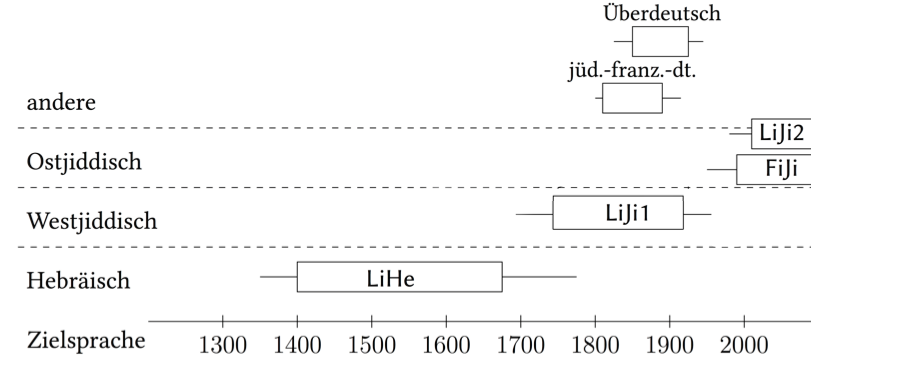
\includegraphics[width=\textwidth]{figures/stadien2.png}
		\caption{\label{stadien} Stadien jüdischer Figurenrede in der deutschsprachigen Literatur}
		\end{figure}



\noindent Wir sehen, dass die sprachliche Markierung jüdischer Rollen in der deutschsprachigen Literatur eine sehr lange Tradition hat. Wie sich die verschiedenen Rollen im Laufe der Zeit gewandelt haben und wie sich 
% dabei 
%\todo{rephrase}
mit ihnen 
die Funktionen der sprachlichen Markierung gewandelt haben, wird diese Arbeit nicht zeigen können. Mit der detaillierten Analyse des \hai{{\LiJi}1} fängt diese Arbeit zumindest einen \,%rs einen
Detailausschnitt aus dem Gesamtbild jüdischer Figurenrede und ihrer \,%rs +r
Funktionen und Formen im literarischen Diskurses zwischen 1700 und dem frühen \,%rs frühen
20. Jahrhundert ein. 



\chapter{Der Nutzen des Literaturjiddischen für die Sprachwissenschaft}\label{lijisprachwissenschaft}

%\epigraph{\begin{flushright}\RL{מיר ווייסן צו ווינציק וועגן מער{ב\makebox(-0.8,9)[r]{\libertineGlyph{uni207B}}}דיקן {{יי}\makebox(-1.5,-5.5)[r]{\libertineGlyph{afii57807}}}דיש, א\makebox(-1.5,-7.5)[r]{\libertineGlyph{uni207B}}ז מיר ז{א\makebox(-1.25,-1.25)[r]{\libertineGlyph{uni05B8}}}לן קענען מוותּר ז{יי}\makebox(-1.5,-7.5)[r]{\libertineGlyph{uni207B}}ן א\makebox(-1.5,-7.5)[r]{\libertineGlyph{uni207B}}פֿילו אויף א\makebox(-1.5,-7.5)[r]{\libertineGlyph{uni207B}} ברעקל עווידענץ.}\end{flushright}%LS! als Zitat einbinden 

%\scriptsize{\sem{Wir wissen zu wenig vom Westjiddischen, als dass wir selbst auf ein Stückchen Evidenz verzichten könnten.}}}{--- \textup{\cite[63]{Weinreich1953}}}

\noindent In seinem Übersichtsartikel zu Forschungsstand und Quellenlage des Westjiddischen geht \cite[62--63]{Weinreich1953} ausdrücklich auf literarische Texte nicht-jüdischer Autoren\footnote{\cite[62]{Weinreich1953} schreibt \quji{\RL{די ד{יי}\makebox(-1.5,-2.5)[r]{\libertineGlyph{uni207B}}טשן}} \sem{die Deutschen}, worunter selbstverständlich auch deutsche Juden fallen würden, jedoch zählt er nur Beispiele christlicher Autoren auf und nennt hingegen in den davorstehenden \,%rs ein Wort
Abschnitten (v.a. \citealt[40–42, 46]{Weinreich1953}) literarische Texte jüdischer Autoren als weitere potenzielle Quellen, woraus sich schließen lässt, dass er an dieser Stelle ausschließlich auf die nicht-jüdische Bevölkerung Deutschlands referiert.} als eine potenzielle Quelle zum Westjiddischen ein und betont deren Nutzen zur Gewinnung historischer Sprachdaten. Exemplarisch nennt er die Publikationen Itzig Veitel Sterns (Pseudonym) und das Drama \qu{Unser Verkehr} (1816) von Karl Borromäus Sessa. \citeauthor{Weinreich1953} sieht zwar, dass eine ernsthafte Analyse dieser Texte absurd wirkt, betont aber, dass im Fall des Westjiddischen jede noch so abwegige Quelle wichtig ist:

\begin{quote}
{\begin{flushright}\RL{א\makebox(-1.5,-7.5)[r]{\libertineGlyph{uni207B}}ז עס איז \RL{{פ\makebox(-0.8,8)[r]{\libertineGlyph{uni207B}}}}א\makebox(-1.5,-7.5)[r]{\libertineGlyph{uni207B}}רא\makebox(-1.5,-7.5)[r]{\libertineGlyph{uni207B}}ן נ{א\makebox(-1.25,-1.25)[r]{\libertineGlyph{uni05B8}}}ך א\makebox(-1.5,-7.5)[r]{\libertineGlyph{uni207B}} \RL{{פ\makebox(-0.8,9)[r]{\libertineGlyph{uni207B}}}}{א\makebox(-1.25,-1.25)[r]{\libertineGlyph{uni05B8}}}נד מקורים וועגן מער{ב\makebox(-0.8,9)[r]{\libertineGlyph{uni207B}}}דיקן {{יי}\makebox(-1.5,-5.5)[r]{\libertineGlyph{afii57807}}}דיש, וו{א\makebox(-1.25,-1.25)[r]{\libertineGlyph{uni05B8}}}ס כ{א\makebox(-1.25,-1.25)[r]{\libertineGlyph{uni05B8}}}טש אונדזער ערשטע רעא\makebox(-1.5,-7.5)[r]{\libertineGlyph{uni207B}}קציע איז \quji{מוקצה}, קענען מיר זיך \RL{{פ\makebox(-0.8,9)[r]{\libertineGlyph{uni207B}}}}{א\makebox(-1.25,-1.25)[r]{\libertineGlyph{uni05B8}}}רט דער\RL{{פ\makebox(-0.8,8)[r]{\libertineGlyph{uni207B}}}}ון ניט {א\makebox(-1.25,-1.25)[r]{\libertineGlyph{uni05B8}}}{פ\makebox(-1,4)[r]{\libertineGlyph{afii57807}}}ז{א\makebox(-1.25,-1.25)[r]{\libertineGlyph{uni05B8}}}גן.}  \end{flushright}}


{\begin{flushright}\LR{\cite[62]{Weinreich1953}}  \end{flushright}}
{\LR{\textit{\footnotesize{az es is faran nokh a fond mekoyrem vegn meyrevdikn yidish, vos khotsh undzer ershte reaktsie iz \qu{muktse}, kenen mir zikh fort derfun nit opzogn.}} }}\\
\LR{\footnotesize{\sem{Es gibt noch weitere Quellen zum Westjiddischen, zu denen zwar unsere erste Reaktion \qu{unbrauchbar} ist, von denen wir uns aber nicht lossagen können.}}} 
\end{quote}



 Der primäre Nutzen einer gezielten und umfangreichen Untersuchung literaturjiddischer Texte nicht-jüdischer Autoren liegt darin zu prüfen, wie geeignet diese als Quellen  des Westjiddischen sind und was sie uns über das Westjiddische und dessen Sprachsituation verraten können.

Doch Weinreichs \isi{Artikel} zur westjiddischen Forschungsagenda bleibt, trotz doppeltem Abdruck, lange Zeit unberücksichtigt. \cite{Althaus1981} ist die einzige Arbeit zur jüdischen Figurensprache mit einem linguistisch-jiddistischen Hintergrund. Obzwar dieser darin autochthone jiddische Strukturen aufzeigt, kommt er zu dem Schluss, dass es sich dabei lediglich um pervertiertes Jiddisch handelt. \cite{Weinreich1953} wird keine Beachtung geschenkt. Die literaturwissenschaftliche Arbeit Richters (\citeyear[insbes.\,99–113]{Richter1995}) äußert die Vermutung, dass die Formen des Literaturjiddischen nicht bloß der Phantasie der Autoren geschuldet sind, sondern tatsächliche Sprachrealitäten abbilden. 

Jedoch sind die Arbeiten von  \cite{Althaus1981} und \cite{Richter1995}\footnote{\citeauthor{Richter1995} analysiert immerhin elf Quellen gründlich, darunter auch das von \cite[62]{Weinreich1953} angeführte Theaterstück \qu{Unser Verkehr} (1816), jedoch steht bei ihm die literaturwissenschaftliche Analyse im Vordergrund.} auf eine nur sehr kleine Auswahl an Texten beschränkt. Auch steht die sprachwissenschaftliche Analyse nicht im Zentrum dieser Untersuchungen. Hinzu kommt, dass in den vergangenen Jahren erste Arbeiten erschienen sind, die den Versuch unternehmen, das Westjiddische des (langen) 19. Jahrhunderts aus den überlieferten Resten heraus zu rekonstruieren \citep{AptrootGruschka2004,Reershemius2007,Reershemius2014,Schaefer2008,Schaefer2010,Schaefer2013,Schaefer2014,Weisskirchen2011,FleischerSchaefer2012}. Damit ist es erstmals möglich, einen Vergleich zwischen Quellen jüdischer und nicht-jüdischer Autoren anzustellen.


\section{Natürliche, konstruierte und fiktionale Sprachen}\label{kunstsprachen}
 \largerpage %longdistance
Um das Verhältnis zwischen \ili{Literaturjiddisch} und gesprochenem \ili{Westjiddisch} zu verstehen, muss man sich der Verhältnisse zwischen fiktionalen, natürlichen und konstruierten Sprachen bewusst werden. Der Begriff \quein{fiktionale Sprache} steht hier entsprechend dem englischen \quein{fictional language} für Sprachen, die ausschließlich innerhalb eines künstlichen Mediums (Literatur, Film) realisiert sind. Mit dieser medialen Fixiertheit unterscheiden sich fiktionale Sprachen von \quein{natürlichen Sprachen}, die sich dadurch auszeichnen, dass sie muttersprachlich erworben werden (\hai{L1}; \hai{N1}-Sprachen in der Diktion von  \citealt[90]{Weiss2001}) und das Potenzial zur Variabilität haben.\footnote{D.\,h. strukturelle Viskosität gegeben ist, vgl.\, S.\, \pageref{viskoserstemal}.} Fiktionale Sprachen sind ein Untertyp von \quein{konstruierten Sprachen}. Konstruierte Sprachen haben die Eigenschaft, dass sie nur als Zweitsprache (\hai{L2}; \hai{N2}-Sprachen nach \citealt[90]{Weiss2001}) erworben werden können, nur beschränkte Variabilität besitzen (und keine viskosen Strukturen haben, s.u.). Zu ihnen zählen formale Sprachen wie Programmiersprachen, aber auch Sprachkonzepte bzw. Metasprachen, die in Grammatiken und Regelwerken festgelegt sind, oder Plan-, Geheim- und Sondersprachen. Da Standardsprachen überwiegend präskriptive Sprachkonzepte sind und auch nie den Gesamtumfang einer natürlichen Sprache erfassen können, fallen sie ebenfalls in die Kategorie formaler, konstruierter Sprachen (vgl.\, \citealt[51]{Chomsky1995}). Das Regelwerk konstruierter Sprachen kann naturalisiert werden, sofern ihre Regeln aktiv angewandt werden und an Kinder als Erstsprache weitergegeben werden, die diese Regeln kreolisieren, wie man es besonders deutlich bei Plan-, Geheim-, Sonder- und Standardsprachen sieht. Eine direkte Beeinflussung fiktionaler Sprachen durch natürliche Sprachen ist z.\,B.\, im Fall des Khuzdul, der Sprache der Zwerge in Tolkiens  \qu{The Hobbit or There and Back Again} (1937) und \qu{The Lord of the Rings} (1954/1955), gegeben, welches sich an semitischen Sprachen (insbes. dem biblischen Hebräischen) orientiert (vgl.\, \citealt[120]{ConleyCain2006}). Eine fiktionale Sprache kann auch den Status einer natürlichen Sprache erlangen. Ein bekanntes Beispiel für den Versuch, aus einer fiktionalen Sprache eine natürliche Sprache zu generieren, sind die bislang gescheiterten Naturalisierungsversuche des Klingonischen der Science-Fiction Reihe \qu{Star Trek} (vgl.\, \citealt{Okrent2010}). Damit  eine fiktionale Sprache sich zu einer natürlichen Sprache entwickeln kann, muss diese jedoch zunächst reglementiert werden. Die meisten fiktionalen Sprachen unterscheiden sich von den übrigen Subtypen konstruierter Sprachen darin, dass sie ursprünglich nicht auf metasprachlich erfassten Regeln beruhen, was in ihrer fiktionalen Funktion begründet ist: Fiktionale Sprache beschränkt sich i.\,d.\,R. auf die Zeichenhaftigkeit selbst. Inhalts- und Ausdrucksseite sind dabei peripher und werden zumeist von der natürlichen Sprache des Mediums etwa durch Übersetzungen oder Untertitel übernommen.

 \largerpage %longdistance
Konstruierte und natürliche Sprachen beeinflussen sich gegenseitig. Exemplarisch lassen sich die ablaufenden Prozesse in den Entwicklungen des Aramäischen nachvollziehen: Zu den Zeiten der Abfassung von Tanach und Talmud waren \ili{hebräisch}-aramäische Varietäten natürliche Sprachen. Durch die jüdische Mehrsprachigkeit der Diaspora verliert das Aramäische an Muttersprachlern, bleibt konserviert als Sakralsprache und entwickelt sich mehr und mehr zu einer konstruierten Sprache, die zwar immer noch als \hai{L2}-Sprache erworben wird, jedoch in der Regel keinen aktiven Gebraucht hat. In manchen Fällen erlangt Hebräisch in der jüdischen Kultur des späten Mittelalters und der frühen Neuzeit sogar den Status einer fiktionalen Sprache, die nur noch innerhalb der Literatur eine Realität besitzt, sprich die Sprache literarisch konserviert ist. Im Zuge des Zionismus des 19. und 20. Jahrhunderts wird mit dem modernen Ivrit eine konstruierte Varietät des Hebräischen entwickelt, die über einen durch politische Umstände geschaffenen muttersprachlichen Erwerb renaturalisiert wurde. Der Theorie Zuckermann (u.\,a.\, \citeyear{Zuckermann2004,Zuckermann2006}) folgend hat jedoch erst der Einfluss natürlicher Sprachen (insbes. des Jiddischen) zur Revitalisierung des Hebräischen im Ivrit als eine fussional-synthetische Sprache beigetragen. Eine Naturalisierung fiktionaler Sprache ist ohne eine rahmenbildende natürliche Sprache nicht möglich.

Für das Literaturjiddische als fiktionale Sprache bleibt zunächst zu klären, ob es sich dabei entweder um ein reines Phantasieprodukt handelt oder ob es auf einer (oder mehreren) natürlichen Sprache(n) beruht. Diese natürliche Sprache wäre idealerweise das Westjiddische, sie kann aber auch ein \qu{intuitives und literarisches Kreolisieren} (\citealt[135]{Haider2007}) des Deutschen, als der Muttersprache nicht-jüdischer Autoren, sein. Mit der emulierenden \isi{Imitation} als Strategie zur Bildung fiktionaler Sprache haben wir es mit einem Sonderfall zu tun. Die daraus resultierenden Medialekte sind eingebunden in eine natürliche Sprache (Matrixsprache). Die Ausdifferenzierung, wo die \isi{Imitation} einsetzt und wo sie aufhört, ist in vielen Fällen problematisch, da hier konstruierte und natürliche Sprache ineinander greifen. Es können daher nur jene Formen als Produkt der Fiktionalisierung gewertet werden, die sich strukturell eindeutig von der Matrixsprache distanzieren. 

\section{Imitation als Feld für psycho- und variationslinguistische Fragestellungen}\label{salienz}
 
Gesetzt den Fall, dass sich die deutschsprachigen Autoren in der Entwickeln des Literaturjiddischen an der tatsächlichen Sprachrealität des Jiddischen orientierten, so lägen uns mit einem \isi{Korpus} dieser fiktionalen Sprache historische Imitationsdaten vor. Ein Quelltyp, der bislang in der Sprachgeschichtsforschung keine Rolle gespielt hat. Bei der \isi{Imitation} rufen Autoren ihre Laienkonzepte des Jiddischen ab. Diese Laienkonzepte können zum einen ihren Ursprung im direkten \isi{Sprachkontakt} zum Jiddischen haben, zum anderen aber auch durch den internen Diskurs um das Jiddische in der deutschsprachigen Literatur und Kultur angeregt und verfestigt worden sein (vgl.\, \citealt[98f]{Richter1995}).   

Doch selbst wenn man davon ausgeht, dass \ili{Literaturjiddisch} in keinem direkten Bezug zum Jiddischen steht, sondern rein konstruiertes Produkt von Muttersprachlern des Deutschen ist, ein \quein{dekonstruiertes Deutsch}, so dürfen wir annehmen, dass diese Sprache den Grundstrukturen germanischer Sprachen unterworfen ist, sofern die Autoren nicht über exzellente Sprachkompetenzen in nicht-germanischen Sprachen verfügen, die sie einfließen lassen. So zeigt Haider (\citeyear{Haider2007}) am Beispiel von Jandls \quein{heruntergekommener Sprache}, dass eine fiktionale Sprache auf Basis des Deutschen vollständig dem entsprechen kann, was in germanischen Sprachen und Kreolisierungen germanischer Sprachen möglich ist. Über emulierende Sprachimitationen können wir damit nicht nur etwas über die zu imitierende Sprache (Zielsprache) lernen, sondern sie zeigen uns vor allem die Möglichkeiten der Matrixsprache (Ausgangssprache).\label{viskoserstemal}

An dieser Stelle möchte ich den Begriff der sprachlichen \quein{Viskosität} einführen, der die potenzielle Flexibilität eines sprachlichen Systems bezeichnet. Je höher die sprachliche Viskosität einer Struktur ist, umso geringer ist ihre Flexibilität, d.\,h. Variabilität. Um ein Beispiel zu nennen, sind etwa germanische \hai{OV}-Sprachen verbsyntaktisch durch eine niedrigere Viskosität gekennzeichnet als germanische \hai{VO}-Sprachen, da erstere deutlich mehr Variation bezüglich der Verbserialisierung aufweisen als letztere (vgl.\, Abschnitt \ref{verbsyntax}, S.\, \pageref{verbsyntax}). Die Positionen, in denen ein sprachliches System besonders geringe Viskosität aufweist, können besonders leicht in emulierenden Imitationen manipuliert werden, ohne starke Verletzungen am System der Matrixsprache vorzunehmen. Hierfür ist der Begriff der \quein{Manipulation} zentral: Die Viskosität eines Systems (\textit{I-Language}) 
bestimmt, wie stark/schwach mögliche Eingriffe (Manipulationen) in das jeweilige System sind. Für das Beispiel der Verbserialisierung heißt dies, dass Abfolgevariationen innerhalb des Verbgefüges in germanischen \hai{OV}-Sprachen mit einer höheren Wahrscheinlichkeit im Bereich der emulierenden \isi{Imitation} manipuliert werden als in \hai{VO}-Sprachen. Dies muss zunächst einmal nicht daran geknüpft sein, wie die Strukturen der Zielsprache tatsächlich aussehen. Die Viskosität einzelner Strukturbereiche einer Sprache können uns auch einen Einblick darin geben, wie und wo Sprachwandel greift bzw. nicht greift. Doch dies ist nur ein Aspekt unter vielen, für den sich die Untersuchung sprachlicher Imitationen als gewinnbringend erweist. 

\isi{Imitation} kann nur stattfinden, wenn eine zu imitierende Sprache bekannt ist (etwa durch direkten oder indirekten \isi{Sprachkontakt}). Da wir den christlichen Autoren des 19. Jahrhunderts eine Kompetenz des Jiddischen weitestgehend absprechen,\footnote{Es mag einzelne Ausnahmen gegeben haben, bei denen eine Teilkompetenz anzunehmen ist, wie etwa die Sondersprachen Lachoudisch im fränkischen Schopfloch (\citealt{Hofmann1998,Klepsch1996,Klepsch2004,Klepsch2008,Matras1996,Philipp1983}) oder Lotegorisch in der Pfalz (\citealt{Meissner1999}) zeigen. Vor allem unter dem Bildungsbürgertum (zumeist Theologen), aber auch unter Händlern nahmen seit dem 16. Jahrhundert die Bestrebungen, Jiddisch zu erlernen, zu (\citealt{Elyada2012}). Wie weit dies jedoch die deutschsprachige Durchschnittsbevölkerung betraf und wie kompetent Christen tatsächlich in der jiddischen Sprache waren, ist schwer zu ermitteln. Für die Literaten des 19. Jahrhunderts kann zwar angenommen werden, dass sie einige Grammatiken der Hebraisten zur Kenntnis genommen haben, die wenigsten unter diesen bieten jedoch eine Basis zum Erlernen des Jiddischen, da i.\,d.\,R. lediglich Hebraismen aufgelistet werden und nur in Ausnahmefällen (z.\,B.\, \citealt{Haselbauer1742,Friedrich1784}) einzelne Beispielsätze angeführt sind. Von modernen Grammatiken zum Zweitspracherwerb sind diese Arbeiten sehr weit entfernt. Bei Konvertiten (\textit{Judenchristen}) sind natürlich Kompetenzen im Jiddischen anzunehmen.} kann angenommen werden, dass die Grundprinzipien der deutschen Grammatik den äußeren Rahmen dieser fiktionalen Sprache bestimmt haben. Hinter der Grundidee der sprachlichen \isi{Emulation} steht auch die Überlegung, dass die Autoren das Jiddische nicht als eigenständige Sprache verstanden haben, sondern es immer im direkten Bezug zum Deutschen wahrnahmen, ähnlich einem deutschen Dialekt (vgl.\, \citealt[127–136]{Elyada2012}). Laienkonzepte werden innerhalb des deutschen Systems emuliert, d.\,h. fremde Strukturen werden an das bestehende System angepasst. Die deutsche Sprache wird manipuliert, um den Effekt des Jiddischen zu erreichen. Die einzelnen Strukturen der Manipulation können uns Aufschluss darüber geben, wie die Laienkonzepte des Jiddischen aussahen, welche wiederum bis zu einem gewissen Grad auch auf die Sprachrealität verweisen.  

Kontaktinduzierte Interferenzen erfassen in erster Linie Strukturen, die vom Basissystem verarbeitet werden können. Demgegenüber nehmen Strukturen weniger Einfluss auf diese Form von Sprachwandel, die auffällig, komplementär anders, \textit{bewusst wahrnehmbar}, im dialektologischen Sinne \textit{salient} sind. Im Fall der Imitation des Jiddischen dienen die sprachlichen Strukturen der Sprachstatik, weil sie das \textit{Eigene} vom \textit{Fremden} bewusst abgrenzen (vgl.\, \citealt[70]{Guenthner2002}). Dies steht komplementär zu den in der Variationslinguistik gängigen Grundüberlegungen vom Zusammenspiel von \quein{Salienz} und \quein{Sprachwandel}, wie sie seit Schirmunskis (\citeyear[118]{Schirmunski1930}) vielmeinenden Ausspruchs die Dialektologie beschäftigen (vgl.\, u.\,a.\, \citealt{HerrgenSchmidt1985,Lenz2010,Elmentaleretal2010,Purschke2011,Purschke2014,Kiesewalter2011,Kiesewalter2014,Hettler2014,Auer2014,Glauninger2014,AndersPalliwodaSchroeder2014,Lorenz2014}): 


\begin{quote}
Wir bezeichnen im weiteren die charakteristischen, d.h. am stärksten auffallenden Abweichungen einer Mundart gegenüber der Schriftsprache (oder anderen Mundarten) als primäre Merkmale, die weniger auffallenden Abweichungen als sekundäre Merkmale. (\citealt[118]{Schirmunski1930})
\end{quote}


Die in dieser Arbeit verwendete Definition von \quein{Salienz} orientiert sich nicht an der dialektologischen Verwendung, die unter \textit{salienten Merkmalen} in der Regel signifikante Merkmale versteht, die bewusst sind. Hingegen bedient sich diese Arbeit eines Salienzbegriffs, wie er u.\,a.\, in Psychologie, Neurologie oder Soziologie üblich ist: Hier bezeichnet \isi{Salienz} die allgemeine Wahrnehmung eines Reizes gegenüber anderen Reizen. Die Wahrnehmung muss dabei nicht auf bewusster Ebene erfolgen, sondern Strukturen  müssen salient sein um bewusst zu werden, d.\,h. wahrnehmbar sein, um bewusst zu werden. Damit eine Struktur bewusst wahrgenommen wird, ist jedoch die Grundvorraussetzung ihre \isi{Salienz}, was jedoch nicht impliziert, dass jede saliente Struktur bewusst wird. Welches sprachliche Merkmal \isi{Salienz} auslöst, ist abhängig vom Grad der typologischen Distanz und Viskosität der Matrixsprache (Ausgangssprache) zur Kontaktsprache und von Grad und Intensität des Sprachkontakts. Nur saliente Strukturen, die verarbeitet werden, können in das System der Matrixsprache aufgenommen werden und dort durch \isi{Emulation} Sprachwandel hervorrufen. Im Rahmen des hier verwendeten Imitationsbegriffs bezeichnet \isi{Salienz} die neuro-kognitive Ebene des \quein{Filters}, der zwischen Zielsprache und Matrixsprache besteht (vgl.\, Abschnitt \ref{begriffsdefinitionen}, S.\, \pageref{emulationsbegriff}). Bewusst wahrgenommene Strukturen können immer nur auf einer Metaebene wirken. Sprachwandel hingegen betrifft das System selbst. Daher kann natürlicher Sprachwandel, d.\,h. Sprachwandel, der nicht durch eine bewusste Sprachlenkung, wie etwa Standardisierung oder Zweitspracherwerb beeinflusst ist, nur bedingt auf salienten Merkmalen aufbauen. Viel wichtiger sind Strukturen, die vom sprachlichen System selbst verarbeitet werden können. Natürlicher Sprachwandel ist in dem Sinne eine Modifizierung des sprachlichen Systems. Die menschliche Fähigkeit zur \isi{Imitation} spiegelt diese Möglichkeit zur Modifikation wider. \isi{Imitation} ist damit nicht ohne Grund der Ausgangspunkt des kindlichen Spracherwerbs (vgl.\, u.\,a.\, \citealt{Uzgiris1981}; \citealt[291–294]{Tauten1997}). Die Imitationsdaten des Literaturjiddischen bieten einen Einblick in diese Strukturen des Sprachkontakts zweier nahverwandter Varietäten. 

Erst die strukturelle Analyse der jüdischen Figurenrede kann die Frage klären, ob es ein allen Texten gemeinsames Konzept vom Literaturjiddischen gab, oder ob jeder Autor seine eigene fiktionale Sprache entwickelte. %Im Fall, dass die Analyse (Abschnitt \ref{analysen}) erstere Annahme bestätigt.\,%rs hier fehlt das weiterführende!
Im Fall eines einheitlichen Literaturjiddischen kann die Vermutung aufgestellt werden, dass Laienkonzepte auf einer einheitlichen Wahrnehmung und Reproduktion sprachlicher Formen natürlicher Sprache fußen. Zugleich spräche dies aber auch dafür, den innerliterarischen Diskurs als Katalysator literaturjiddischer Formen zu verstehen. Würde jeder Autor andere Formen der sprachlichen Markierung verwenden, so ließe sich der literarische Diskurs als Triebfeder ausschließen und erst der Vergleich zu autochthon westjiddischen Quellen kann entscheiden, ob der Autor auf ein Laienkonzept oder seine Phantasie zurückgreift. Ein interessantes Ergebnis wäre, wenn sich das Literaturjiddische regional und nicht idiolektal unterscheiden würde. So ließe sich zum einen darauf schließen, dass die Autoren ihre eigene Dialektalität, sprich dialektales Deutsch, haben einfließen lassen oder aber sogar, dass die westjiddischen Varietäten im Raum streuen und wir somit erstmals dialektale Strukturen erkennen könnten.

  
Das Einfließen deutsch-dialektaler Strukturen in das Literaturjiddische wiederum führt uns in den Bereich der Diglossieforschung (vgl.\, \citealt{Ferguson1959}). Gerade für das 18. und 19. Jahrhundert kann man davon ausgehen, dass die meisten Autoren in einer diglossischen Sprachsituation zwischen Schriftsprache und gesprochener Sprache (Dialekt) standen. Eine Diskrepanz zwischen Schriftlichkeit und Mündlichkeit findet sich bis in die heutige Zeit (vgl.\, \citealt{KochOesterreicher1985}), mit dem Unterschied, dass nun kaum mehr (Basis-)Dialekte, sondern Regiolekte und nicht-arealgebundene Soziolekte die Mündlichkeit ausmachen (vgl.\, \citealt{SchmidtHerrgen2011}). So ist anzunehmen, dass bei dem Versuch, (jiddische) Dialektalität in die literarische Schriftlichkeit zu transponieren, die eigene Umgangssprache einfließt. Aus diesem Grund wird die nachfolgende Analyse auch immer die gewonnenen Daten des Literaturjiddischen mit der Situation in den deutschen Dialekten abgleichen (s. Abschnitt \ref{analysen}). Darüber hinaus funktioniert der Einsatz des Literaturjiddischen ähnlich wie \quein{code-mixing} (vgl.\, \citealt{MyersScotton2004,MyersScotton2002}): jüdische Figuren \textit{sprechen} ein Schriftdeutsch, welches durchsetzt ist mit jiddischen bzw. mit als \quein{jiddisch} verstandenen Elementen.  

Emulierende fiktionale Sprachen wie das \hai{{\LiJi}} können uns darüber hinaus dabei helfen, den kognitiven Aufwand von sprachlicher Rekonstruktion nachzuvollziehen. 
Der Umstand, dass nur bestimmte Formen emuliert werden, ist nicht zwangsläufig autochthonen jiddischen Formen geschuldet, sondern gibt auch Hinweise auf die Struktur unserer Sprachverarbeitung. Dies möchte ich an einem Fallbeispiel illustrieren: Will ein Autor eine jüdische Figur jiddisch sprechen lassen und möchte zusätzlich, dass der Inhalt der Figurenrede für die Leserschaft verständlich ist, hätte er vier Möglichkeiten: 

\begin{itemize}
\item [1.] Verwendung des Jiddischen (erworben durch Grammatiken, Kontakt mit Muttersprachlern o.\,ä.).
\item [2.] Verwendung des Jiddischen (erworben durch Grammatiken, Muttersprachler o.\,ä.) mit paralleler Übersetzung in die Matrixsprache (Deutsch).
\item [3.] Verwendung des Deutschen mit Elementen des Jiddischen (aus eigenem Laienkonzept, welches auf direktem \isi{Sprachkontakt} beruht).
\item [4.] Verwendung des Deutschen mit Elementen des \hai{{\LiJi}} (sofern kein Laienkonzept aus direktem \isi{Sprachkontakt} vorhanden ist).
\end{itemize}

Nur in den Fällen 2, 3 und 4 wäre eine Verständlichkeit des Sprechtexts der jüdischen Figur durch den Leser garantiert. Möglichkeit 1 kann damit ausgeschlossen werden. Da es wohl ein zu hoher Aufwand für einen Autor wäre, sich die jiddische Sprache anzueignen und v.\,a.\, da eine Übersetzung den Lesefluss beeinträchtigen würde, sind keine Texte zu finden, die sich Möglichkeit 2 zunutze machen. Bei den verbliebenen Strategien 3 und 4 ist die Verständlichkeit garantiert, solange emulierte Formen in die Matrixsprache (Deutsch)  rekonstruiert werden können. Dabei muss der Autor/Leser des \hai{{\LiJi}} über die kognitive Fähigkeit verfügen, zu wissen, welche sprachlichen Strukturen sich rekonstruieren bzw. nicht mehr rekonstruieren lassen. Anhand von emulierenden fiktionalen Sprachen ließe sich testen, welche sprachlichen Strukturen höherer Verarbeitungsleistungen bedürfen als andere. Die aus dem \hai{{\LiJi}} gewonnenen Daten könnten so als Grundlage für psychoneurolinguistische Untersuchungen der Wort- und Sprachverarbeitung dienen.

Doch bereits die Formen, die wir im \hai{{\LiJi}} finden, können als positive Evidenz für leicht rekonstruierbare Strukturen interpretiert werden.

Damit bringt eine Analyse des \hai{{\LiJi}} die drei folgenden psycho- und variationslinguistischen Fragestellungen mit sich:

\begin{description}
\item [] i. Was ist in der Matrixsprache (Deutsch) möglich (= d.\,h. was ist überhaupt konstruierbar)?
\item [] ii. Was sagt dies über die typologische Beschaffenheit und Nähe von Zielsprache (Jiddisch) und Matrixsprache (Deutsch) aus?
\item [] iii. Was kann aus dem \hai{{\LiJi}} in die Matrixsprache (Deutsch) rekonstruiert werden (= d.\,h. was ist überhaupt verarbeitbar)?
\end{description} 


 
\section{Literaturjiddisch als Sekundärquelle des späten Westjiddisch}\label{secundärquelle}
 
Die in den Abschnitten \ref{kunstsprachen} und \ref{salienz} dargelegten Prämissen erlauben die Annahme, dass die Sprachrealität des Westjiddischen ihren Niederschlag im Literaturjiddischen gefunden hat. So betrachtet können die zu untersuchenden literarischen Texte als Sekundärquellen zum Jiddischen verstanden werden. Dies ließe sich im Vergleich zu unserem derzeitigen Wissen über das späte \ili{Westjiddisch} (s. Abschnitt \ref{westjiddistik}) prüfen. Für den Fall, dass die literaturjiddischen Quellen tatsächlich Nähe zum Westjiddischen aufweisen, würde dies unsere bisher gewonnenen Daten bestätigen. Darüber hinaus ließen sich aber auch Erweiterungen unseres Wissens erwarten, sofern Strukturen im Literaturjiddischen auftreten, die wir nur vereinzelt in westjiddischen Primärquellen finden. Des Weiteren lassen sich Vermutungen über die Authentizität bisher unbelegter Strukturen machen, sofern diese in den Sekundärquellen wiederholt in Erscheinung treten.

Literaturjiddische Texte können aber auch soziolinguistische Prozesse widerspiegeln. So ist anzunehmen, dass der westjiddische \isi{Sprachtod} im Rückgang westjiddischer Formen im Literaturjiddischen reflektiert wird. Demgegenüber ist ein möglicher Zugewinn ostjiddischer Formen im Verlauf des 19. Jahrhunderts parallel zum kulturellen Aufstieg dieser Sprache und möglicher Migrationsbewegungen von Ostjiddischsprechern in den Westen nicht auszuschließen.

